% =====================================================================
%  Paper 1: what a scene description does in training-free video anomaly
%  detection, and where it fails. Elsevier CAS single-column format (cas-sc).
%  Figures and references.bib are shared with main.tex in this folder.
% =====================================================================

\documentclass[a4paper,fleqn]{cas-sc}

% Numbered citation style, matching model1-num-names.bst shipped with the CAS
% bundle (and the convention of Pattern Recognition Letters / Neurocomputing).
% \citep gives [12]; \citet gives "Liu et al. [12]" -- both still work.
% To switch to author-year instead: use [authoryear,longnamesfirst] here and
% \bibliographystyle{cas-model2-names} at the end (that .bst must be present).
\usepackage[numbers,sort&compress]{natbib}

% cas-sc already provides: geometry, graphicx, hyperref, xcolor, natbib
% hooks, and enhanced enumerate/itemize. Do NOT load those again.
% Graphics are searched for beside this file and in figures/, so a plain
% \includegraphics{name} resolves either way: flat, as the files sit in the
% Overleaf project, or in the figures/ subdirectory, as they sit in the repo.
% Keep the calls unprefixed -- adding "figures/" back would break the flat case.
%
% The calls also carry NO file extension, deliberately. Under pdflatex graphicx
% tries .pdf before .png, so the vector version of a figure is used wherever one
% exists and the raster one is the automatic fallback where it does not. Every
% figure used to be raster at 400dpi, which is ample for print yet still reads
% as soft on screen, because a viewer at 175% zoom resamples a bitmap while
% vector text does not resample at all. scripts/make_*.py now emit both forms;
% upload the .pdf alongside the .png and the report picks it up with no edit.
\graphicspath{{./}{figures/}}

\usepackage{amsmath,amssymb}
\usepackage{booktabs}
\usepackage{tabularx}
% rotating: the architecture figure sits on its own landscape page, where the
% text height is the available width, so it prints at full size and stays legible
\usepackage{rotating}
\usepackage{algorithm}
\usepackage{algpseudocode}

% cas-sc emits the first-page "ORCID(s):" footnote heading unconditionally, so
% it still prints -- empty -- once every \author has no orcid option. This
% silences the macro that produces it. Guarded with \@ifundefined so the build
% is unaffected if a future class version renames or drops it.
% REMOVE THIS BLOCK once the authors have ORCIDs and the line should appear.
\makeatletter
\@ifundefined{printorcid}{}{\renewcommand{\printorcid}{}}
\makeatother

% ---------- float placement ----------
% The paper has 23 tables and 11 figures. LaTeX's defaults allow floats to fill
% little of a page, so they queue up and drift to the end; these settings let a
% page carry more float and keep each table near its first mention.
\renewcommand{\topfraction}{0.9}
\renewcommand{\bottomfraction}{0.8}
\renewcommand{\textfraction}{0.07}
\renewcommand{\floatpagefraction}{0.7}
\setcounter{topnumber}{3}
\setcounter{bottomnumber}{2}
\setcounter{totalnumber}{5}

% ---------- table column types ----------
% cas-sc defines L, C and R itself, so ours use different letters.
% Z         : ragged-right stretchable column (tabularx)
% W{width}  : fixed-width ragged-right paragraph column
\newcolumntype{Z}{>{\raggedright\arraybackslash}X}
\newcolumntype{W}[1]{>{\raggedright\arraybackslash}p{#1}}

% =====================================================================
\begin{document}
\let\WriteBookmarks\relax
\def\floatpagepagefraction{1}
\def\textpagefraction{.001}

\shorttitle{What a scene description does in training-free video anomaly detection}
\shortauthors{P. K. Sarangi et~al.}

\title[mode = title]{Concept Shift in Training-Free Video Anomaly Detection: What
a Scene Description Does, and Where It Fails}

\author[1]{Prakash Kumar Sarangi}
% \cormark[1]
% \ead{prakash_m251250cs@nitc.ac.in}
\credit{Conceptualization, Methodology, Software, Investigation, Formal analysis,
Writing -- original draft}

\affiliation[1]{organization={National Institute of Technology Calicut},
    addressline={Department of Computer Science and Engineering},
    city={Kozhikode},
    postcode={673601},
    state={Kerala},
    country={India}}

\author[1]{Pranesh Das}
\credit{Supervision, Conceptualization, Writing -- review and editing}

\author[1]{Raju Hazari}
\credit{Supervision, Writing -- review and editing}

% \cortext[cor1]{Corresponding author}

\begin{abstract}
Training-free video anomaly detection scores frames against text with frozen
vision-language models, promising one detector for many cameras. We ask what a natural-language description of the scene
contributes to such a detector. We first argue that anomaly detection is dominated
by \emph{concept shift}---the same input labelled differently in different
places---which the domain-adaptation literature deliberately sets aside. We then
build a fully frozen pipeline (CLIP ViT-L/14, prompt ensembles, temporal smoothing)
in which the description is the only quantity that varies, so its effect is
identifiable, and test it with a protocol whose mismatched condition can falsify
the claim. On ShanghaiTech the predicted signature appears only when the description
enters the normal prompt ensemble alone; adding it to both ensembles draws the
prototypes together and reverses the effect (matched minus mismatched moves from
$-0.029$ to $+0.105$). The effect nearly vanishes on single-camera CUHK Avenue and
within single ShanghaiTech views, and per-camera descriptions generated by a frozen
LLaVA model reach $0.751$ AUROC with no human input. On UCF-Crime, under predictions
registered before scoring, per-video descriptions reach $0.824$ $[0.756, 0.877]$,
comparable to LAVAD and AnyAnomaly, and beat other videos' descriptions by $+0.110$
$[+0.069, +0.157]$. A pre-specified audit attributes $82$--$87\%$ of these gains to
per-video calibration rather than to re-ranking frames. Two further benchmarks bound
the method: on XD-Violence the generated description lowers average precision from
$0.624$ to $0.417$, because in 127 of 500 violent videos the frames it is written
from already show the event, and on NWPU Campus it has no measurable effect.
\end{abstract}

\begin{highlights}
\item Anomaly detection is dominated by concept shift, which domain adaptation sets aside
\item A fully frozen detector makes a scene description's effect identifiable
\item Adding the description to both prompt ensembles reverses its effect
\item The description mainly calibrates cameras: 82--87\% of gains are level shifts
\item It fails when written from frames that already show the anomaly
\end{highlights}

\begin{keywords}
video anomaly detection \sep concept shift \sep domain adaptation \sep
vision-language models \sep training-free detection \sep scene context
\end{keywords}

\maketitle

\section{Introduction}
\label{sec:intro}

Anomaly detection identifies rare, unexpected events in images or video and
underpins applications from industrial inspection to public-space surveillance.
The dominant formulation is one-class learning: a model of ``normal'' is estimated
from a large corpus of normal samples, and departures from it are flagged. This
carries a cost that motivates the present work. The learned notion of normality is
bound to the environment in which it was estimated, so a change of camera, site or
application invalidates the model, and recovering performance requires fresh data
collection and retraining for every deployment.

That cost is conventionally addressed by \emph{domain adaptation} (DA). We observe
that the DA literature and the anomaly detection setting are misaligned in a
specific way. Domain shift decomposes into several types, and the DA literature
concentrates---by explicit scoping decision---on \emph{covariate shift}, a change in
the input distribution. In anomaly detection, normality is defined by the deployment
context rather than by object identity, so the same visual content can be normal in
one environment and anomalous in another: a vehicle on a road and on a pedestrian
walkway. That is \emph{concept shift}, the type the literature sets aside
(Section~\ref{sec:gap}).

A second development sharpens the mismatch. Vision-language models trained at web
scale, such as CLIP \citep{radford2021clip}, recognise concepts specified in
natural language, and the breadth of their training makes them robust to much of
the appearance variation that covariate-shift methods were built to correct. If a
foundation model already absorbs much of the covariate shift, what remains is
precisely the shift the field excluded. A natural response is to tell the model, in
words, where it is.

This paper examines that response under conditions in which its effect can be
measured. We build a video anomaly detector in which every model is frozen and the
only quantity that varies between deployments is a short description of the scene.
Because no parameter is updated anywhere, a difference in output between two runs
that differ only in the description is attributable to the description. We pair the
detector with a protocol that varies only that text, including a deliberately wrong
description that would refute the claim if it cost nothing. The findings are mixed,
and we report them as they fell: the description is load-bearing, but where it is
injected matters more than what it says; it needs several scenes to help; it acts
mainly by calibrating cameras against one another; and on two further benchmarks it
fails, once because it describes the anomaly as normal.

\section{Related Work}
\label{sec:lit}
\subsection{Zero-shot and training-free anomaly detection}
Vision-language models (VLMs) trained on web-scale image--text corpora, notably
CLIP \citep{radford2021clip}, permit classification of concepts specified purely
in natural language. WinCLIP \citep{jeong2023winclip} applied this to industrial
anomaly detection by scoring images against ensembles of ``normal'' and
``abnormal'' text prompts, requiring no task-specific training; AnomalyCLIP
\citep{zhou2024anomalyclip} learns object-agnostic prompts to improve
generalisation across categories. These are evaluated primarily on MVTec~AD
\citep{bergmann2019mvtec}, against trained baselines such as PatchCore
\citep{roth2022patchcore}.

In video, LAVAD \citep{zanella2024lavad} demonstrated fully training-free VAD by
captioning frames with a VLM, scoring caption sequences with a large language
model, and refining the result via cross-modal similarity. VERA
\citep{ye2025vera} keeps the VLM frozen and instead learns a set of verbal
\emph{guiding questions}, yielding explainable detection; notably, these
questions are optimised offline on source data, so the adaptation is not
performed at test time. AnyAnomaly \citep{anyanomaly2025} lets a user define the
anomaly of interest in text at inference time, and OVVAD \citep{wu2024ovvad}
addresses the open-vocabulary setting using frozen CLIP encoders, a nearly
weight-free temporal adapter, and detection and classification heads trained
on the benchmark's training videos.

More recent training-free methods concentrate on the text side.
NOVA \citep{yin2026nova} constructs normal and anomalous prompt banks per anomaly
class and forbids look-alike actions from the normal side; ASK-Hint
\citep{zou2026askhint} shows that action-centric prompts elicit better judgements
from frozen vision-language models than abstract labels; Flashback
\citep{lee2025flashback} retrieves from a large memory of generated captions. None of
these isolates the contribution of a description of the deployment scene, which is
the question addressed here.

\subsection{Domain adaptation: the classical view}
Domain adaptation is the subfield of transfer learning in which the task is
fixed and the data distribution changes. The literature is mature and well
surveyed. \citet{patel2015visual} review the shallow era---subspace alignment,
geodesic-flow interpolation between source and target subspaces, dictionary
learning, and projection of heterogeneous features into a shared latent space.
\citet{wang2018deep} provide the canonical deep taxonomy. They divide one-step
DA into three families. \emph{Discrepancy-based} methods minimise a measured
gap between the domains. \emph{Adversarial-based} methods train a feature
extractor to defeat a domain discriminator, so that the features it produces
carry no domain signal. \emph{Reconstruction-based} methods use reconstruction
as an auxiliary task that encourages invariance. Where source and target are too
far apart to bridge in one step, multi-step DA constructs intermediate domains
between them.

\citet{wilson2020survey} organise unsupervised DA by mechanism---domain-invariant
feature learning, domain mapping, normalisation statistics, ensembles,
target-discriminative methods---and decompose methods into interchangeable
components, alongside the generalisation bound that motivates divergence
minimisation. \citet{liu2022deep} survey modern unsupervised DA:
statistic alignment, adversarial learning, generative mapping, self-training and
self-supervision, applied across natural images, medical imaging, video,
language and time series. They also list open directions, among them
source-free adaptation, continuous and test-time adaptation, and adaptation in
the foundation-model era. \citet{singhal2023domain} consolidate the field,
stating the theoretical conditions under which DA is justified and categorising
settings by label-set relationship (closed-set, partial, open-set, universal).

\subsection{Domain adaptation beyond vision}
The mechanism of adaptation changes substantially in the language-model era.
\citet{fan2026llm} review large language model adaptation for geotechnical
engineering. They describe four strategies forming ``a continuum balancing cost,
complexity, and performance'': \emph{prompt engineering},
\emph{retrieval-augmented generation}, \emph{domain-adaptive pretraining} and
\emph{fine-tuning}. The two ends of that continuum matter here. Prompt
engineering is the cheapest and most immediate, but ``often lacks depth and
robustness''; fine-tuning gives the highest task precision at the highest cost
in compute and labels.
The relevant structural observation is that in this paradigm the model may remain
unchanged while the \emph{input context} carries the adaptation---a category
absent from the visual DA taxonomies above, which predate foundation models.

\subsection{Domain adaptation within video anomaly detection}
Work applying DA specifically to VAD falls into three groups, distinguished by
what the target domain costs. \emph{Learned adaptation} requires target data and
a training run: Ada-VAD \citep{adavad2024} pretrains a domain-invariant predictor
with synthesised abnormal samples and then adapts adversarially to a few target
frames. \emph{Meta-learned scene adaptation} reduces but does not remove that
cost: \citet{lu2020fewshot} meta-train across many scenes so that a
future-frame-prediction model adapts to an unseen scene from a handful of frames.
\emph{Zero-shot cross-domain} methods remove the target-time cost entirely: zxVAD
\citep{aich2023zxvad} performs cross-domain VAD without any target adaptation,
contrasting normal features against pseudo-anomalies synthesised by an untrained
network.

Two properties are common to all three. First, each still trains a model on
source data, so the notion of normality is fixed by source visual statistics.
Second, and decisively for the present work, none provides a channel through
which an operator can \emph{state} what normality means in the target
environment; adaptation is mediated entirely by pixels and parameters, never by
language.

\subsection{Summary of the reviewed literature}
\label{sec:lit-summary}
Tables~\ref{tbl:lit-da}, \ref{tbl:lit-vad} and~\ref{tbl:lit-vad2} summarise the works reviewed above:
for each, its venue and year, its central idea, the challenge or limitation that
matters for the present problem, and the scope it leaves for further work. The
last two columns are read from the standpoint of this paper, a training-free
detector that must adapt to a new scene without target data; where a work states
its own open directions, those are given.

\begin{table}[width=\linewidth,cols=6,pos=htbp]
\caption{Domain adaptation literature reviewed in Section~\ref{sec:lit}.}
\label{tbl:lit-da}
\footnotesize
\begin{tabularx}{\linewidth}{@{}W{2.1cm} l W{1.7cm} Z Z Z@{}}
\toprule
\textbf{Work} & \textbf{Year} & \textbf{Venue} & \textbf{Key idea} &
\textbf{Challenge / limitation} & \textbf{Future scope} \\
\midrule
Patel et al. \citep{patel2015visual} & 2015 & IEEE Signal Process.\ Mag. &
Survey of shallow visual DA: subspace alignment, geodesic-flow interpolation,
dictionary learning, shared latent spaces &
Hand-crafted features; target data needed; labelling function assumed common to
both domains &
Deep and label-efficient adaptation \\
\addlinespace
Wang and Deng \citep{wang2018deep} & 2018 & Neurocomputing &
Deep DA taxonomy: discrepancy-, adversarial- and reconstruction-based methods;
multi-step DA for distant domains &
Every family trains on target samples; aligns the input distribution only &
Adaptation without target training \\
\addlinespace
Kouw and Loog \citep{kouw2018introduction} & 2018 & arXiv &
Formal taxonomy of shift: covariate, conditional, label and concept shift &
Concept shift defined but left largely without methods &
Methods for shift in $p(y \mid x)$ \\
\addlinespace
Wilson and Cook \citep{wilson2020survey} & 2020 & ACM Comput.\ Surv. &
Unsupervised deep DA organised by mechanism, with the generalisation bound that
motivates divergence minimisation &
The bound presumes a small joint error, in effect a shared labelling function &
Settings where that presumption fails \\
\addlinespace
Liu et al. \citep{liu2022deep} & 2022 & APSIPA Trans.\ Signal Inf.\ Process. &
Review of modern unsupervised DA: statistic alignment, adversarial, generative,
self-training &
Scope explicitly restricted to covariate shift; concept shift set aside &
Stated by the authors: source-free, continual and test-time DA, and DA for
foundation models \\
\addlinespace
Singhal et al. \citep{singhal2023domain} & 2023 & IEEE Access &
Consolidates the theory and settings of DA (closed-set, partial, open-set,
universal) &
Lists covariate shift, $P(Y_s \mid X_s) = Q(Y_t \mid X_t)$, as a condition for DA
&
Adaptation when that condition is violated \\
\addlinespace
Fan et al. \citep{fan2026llm} & 2026 & Solid Earth Sci. &
LLM adaptation as a cost--performance continuum: prompting, retrieval, adaptive
pre-training, fine-tuning &
Prompting is cheapest but ``often lacks depth and robustness''; language only &
Prompt-level adaptation for vision models \\
\addlinespace
Wilkinghoff et al. \citep{wilkinghoff2026context} & 2026 & arXiv &
Position: normality depends on operating context; fixed normality creates
``structural ambiguity'' &
Position paper, no method; context from additional sensors &
Conditional anomaly assessment, measured \\
\bottomrule
\end{tabularx}
\end{table}

\begin{table}[width=\linewidth,cols=6,pos=htbp]
\caption{Anomaly detection literature reviewed in Section~\ref{sec:lit}, in order
of year, 2020--2024 (continued in Table~\ref{tbl:lit-vad2}). DA: domain
adaptation; VAD: video anomaly detection; VLM: vision-language model.}
\label{tbl:lit-vad}
\footnotesize
\begin{tabularx}{\linewidth}{@{}W{2.1cm} l W{1.2cm} Z Z Z@{}}
\toprule
\textbf{Work} & \textbf{Year} & \textbf{Venue} & \textbf{Key idea} &
\textbf{Challenge / limitation} & \textbf{Future scope} \\
\midrule
Lu et al. \citep{lu2020fewshot} & 2020 & ECCV &
Meta-learned scene adaptation of a frame-prediction model from a few frames &
Trains on source scenes; needs target frames and an update &
Adaptation with no target update \\
\addlinespace
CLIP \citep{radford2021clip} & 2021 & ICML &
Contrastive image--text pre-training; zero-shot classification from text &
One embedding per image at $224\times224$; small objects lost &
Region- and patch-level use for anomalies \\
\addlinespace
zxVAD \citep{aich2023zxvad} & 2023 & WACV &
Cross-domain VAD with no target adaptation; pseudo-anomalies from an untrained
network &
Normality fixed by source visual statistics; no way to state target normality &
Operator-specified normality \\
\addlinespace
WinCLIP \citep{jeong2023winclip} & 2023 & CVPR &
Zero-shot anomaly detection with normal/abnormal prompt ensembles and windowed
scoring &
Industrial images; normality not tied to a scene &
Video and scene-dependent normality \\
\addlinespace
Ada-VAD \citep{adavad2024} & 2024 & SDM &
Domain-invariant predictor with synthesised anomalies, adapted adversarially to a
few target frames &
Target data and a training run per deployment &
Training-free adaptation \\
\addlinespace
AnomalyCLIP \citep{zhou2024anomalyclip} & 2024 & ICLR &
Learns object-agnostic prompts for zero-shot anomaly detection &
Prompt learning needs auxiliary labelled data &
Fully training-free prompting \\
\addlinespace
LAVAD \citep{zanella2024lavad} & 2024 & CVPR &
Training-free VAD: frame captions scored by an LLM, refined by cross-modal
similarity &
Chains a captioner, an LLM and a refiner; scene context not isolated &
Lighter scoring; the role of context \\
\addlinespace
OVVAD \citep{wu2024ovvad} & 2024 & CVPR &
Open-vocabulary VAD with frozen CLIP, a light temporal adapter and trained heads &
Heads trained on the benchmark's training videos &
Zero-shot transfer to new scenes \\
\bottomrule
\end{tabularx}
\end{table}

\begin{table}[width=\linewidth,cols=6,pos=htbp]
\caption{Anomaly detection literature reviewed in Section~\ref{sec:lit}
(continued), 2024--2026.}
\label{tbl:lit-vad2}
\footnotesize
\begin{tabularx}{\linewidth}{@{}W{2.1cm} l W{1.2cm} Z Z Z@{}}
\toprule
\textbf{Work} & \textbf{Year} & \textbf{Venue} & \textbf{Key idea} &
\textbf{Challenge / limitation} & \textbf{Future scope} \\
\midrule
AnomalyRuler \citep{yang2024anomalyruler} & 2024 & arXiv &
An LLM induces rules of normality from a few normal frames, then reasons over them &
Needs normal target frames and GPT-4 &
Rule induction without target frames \\
\addlinespace
Flashback \citep{lee2025flashback} & 2025 & arXiv &
Zero-shot, real-time VAD by retrieval from a memory of generated captions &
Contribution of the deployment scene not isolated &
Scene-aware memories \\
\addlinespace
VERA \citep{ye2025vera} & 2025 & CVPR &
Frozen VLM guided by verbal questions learned on training data; explainable &
Questions optimised offline on labelled data; explanations under shift
unmeasured &
Explanation quality under domain shift \\
\addlinespace
AnyAnomaly \citep{anyanomaly2025} & 2026 & WACV &
Customisable VAD: the user names the anomaly; three large-VLM queries per segment &
The anomaly classes must be named in advance; heavy inference &
Detection of unnamed anomalies \\
\addlinespace
ASK-Hint \citep{zou2026askhint} & 2026 & WACV &
Action-centric, fine-grained prompts elicit better judgements from frozen VLMs &
Contribution of the deployment scene not isolated &
Scene-conditioned prompting \\
\addlinespace
NOVA \citep{yin2026nova} & 2026 & arXiv &
Normal and anomalous prompt banks per anomaly class; look-alike actions barred
from the normal side &
Banks written per anomaly class; scene context not isolated &
Normal-side modelling without class lists \\
\addlinespace
Song and Lee \citep{song2026vlmanswer} & 2026 & arXiv &
A VLM's answer is not an anomaly score: yes/no outputs compress rankings &
Concerns score design, not adaptation &
Calibrated, rank-preserving scores \\
\bottomrule
\end{tabularx}
\end{table}

\section{Concept Shift and the Research Gap}
\label{sec:gap}
% =====================================================================

\subsection{Observation 1: the field targets covariate shift by design}
A domain is a joint distribution $P(x,y) = P(y\mid x)\,P(x)$, and shift may occur
in any factor. Following the taxonomy of \citet{kouw2018introduction} as
presented by \citet{liu2022deep}, four types are distinguished, summarised in
Table~\ref{tbl:shifts}.

\begin{table}[width=\linewidth,cols=3,pos=htbp]
\caption{The four types of domain shift.}\label{tbl:shifts}
\begin{tabularx}{\linewidth}{@{}l W{2.6cm} Z@{}}
\toprule
\textbf{Shift type} & \textbf{Factor} & \textbf{Standard example} \\
\midrule
Covariate shift        & $p(x)$       & Same objects under a different camera, lighting, or weather \\
Conditional shift      & $p(x\mid y)$ & A class appears differently across domains \\
Label / target shift   & $p(y)$       & Class proportions differ between domains \\
\textbf{Concept shift} & $p(y\mid x)$ & \textbf{The same input carries a different label} (a tomato classified as a vegetable in one country and a fruit in another) \\
\bottomrule
\end{tabularx}
\end{table}

\citet{liu2022deep} state their scope explicitly: concept shift ``is, however,
usually not a common problem in popular object classification or semantic
segmentation tasks. As such, this review mainly focuses on the covariate shift
alignment in UDA, as is most commonly studied,'' listing the remaining shifts as
directions for future research. Consistently, \citet{singhal2023domain} give
covariate shift---$P(Y_s\mid X_s) = Q(Y_t\mid X_t)$---as the first theoretical
condition under which DA is justified, which is to say that classical DA theory
\emph{assumes concept shift away}.

\subsection{Observation 2: anomaly detection is concept-shift dominated}
In anomaly detection, normality is a property of the deployment context rather
than of the object. Table~\ref{tbl:conceptshift} gives three cases in which the
visual content is unchanged while the correct label inverts with the domain.

\begin{table}[width=\linewidth,cols=4,pos=htbp]
\caption{Concept shift in video anomaly detection. The third case is an actual
anomaly class in the ShanghaiTech benchmark \citep{liu2018shanghaitech}.}
\label{tbl:conceptshift}
\begin{tabularx}{\linewidth}{@{}Z l l l@{}}
\toprule
\textbf{Input $x$} & \textbf{Domain A} & \textbf{Domain B} & \textbf{Shift} \\
\midrule
A person running    & park: normal   & bank vault: anomalous        & $p(y\mid x)$ \\
A person lying down & beach: normal  & factory aisle: anomalous     & $p(y\mid x)$ \\
A vehicle           & road: normal   & walkway: anomalous           & $p(y\mid x)$ \\
\bottomrule
\end{tabularx}
\end{table}

These are concept shift by definition. Methods that align $p(x)$ cannot address them. That family is
the dominant one across \citet{wang2018deep}, \citet{wilson2020survey} and
\citet{liu2022deep}, and it is the wrong instrument here: $p(x)$ may be identical
across the two domains while only the labelling function differs.

\citet{wilkinghoff2026context} reach the same conclusion independently. They
observe that ``a specific observation may be normal under one operating
condition, yet anomalous under another'', and argue that judging such an
observation against a single fixed notion of normality creates what they term
``structural ambiguity''. Abnormality, they conclude, should be assessed
conditionally.

We read that agreement as support for the premise rather than as competition
for it. Three things separate the two accounts. First, we state the problem in
the vocabulary of the domain-adaptation literature, which is what makes the
mismatch in Observation~1 visible: the shift anomaly detection exhibits is the
one that literature sets aside. Second, their context arrives through additional
sensing modalities, whereas ours arrives as a sentence written by an operator
and needs no extra instrumentation. Third, their paper is a position: it argues
for conditional assessment and lists open problems. This work supplies a
mechanism, and a protocol that can establish whether the supplied context does
anything at all.

\subsection{Observation 3: foundation models relocate the problem}
\citet{liu2022deep} pose the foundation-model question directly and answer it in
part: such models ``are robust to the covariate shift in many cases,'' but ``it
is challenging to alleviate the label shift, without access to target domain
data. In addition, the concept shift can also cause a problem, even though there
are sufficient training data.'' A frozen CLIP encoder has been exposed to an
enormous diversity of cameras, lighting conditions, and viewpoints, so much of
the covariate shift that classical DA was constructed to correct is already
absorbed. What remains is precisely the shift the literature set aside.

\subsection{Statement of the research gap}
\begin{enumerate}[G1.]
  \item \textbf{Concept shift dominates VAD but is unstudied as such.} The DA
        literature scopes it out as uncommon; in VAD it is the primary shift.
        That normality is context-dependent has recently been argued
        \citep{wilkinghoff2026context}, but not in the vocabulary that locates
        the mismatch: no existing work states VAD domain shift in the DA
        literature's own taxonomy, where the exclusion becomes visible.
  \item \textbf{No protocol measures language-mediated adaptation.} The standard
        DA protocol compares source-trained against target-adapted accuracy,
        which presupposes a training step. There is no established way to test
        whether a \emph{description} adapted anything.
  \item \textbf{Foundation-model-era DA is empirically under-characterised.}
        Identified as an open direction by \citet{liu2022deep}, with little
        empirical evidence on which shifts a frozen VLM absorbs unaided.
  \item \textbf{Explanation quality under domain shift is unexamined.} None of
        the six DA surveys addresses it. Explainable VAD \citep{ye2025vera}
        transfers its learned questions across datasets, but reports detection
        AUC there; whether the explanations remain correct under shift is not
        measured.
\end{enumerate}

\section{Contributions}
\label{sec:contrib}

\begin{enumerate}[C1.]
  \item \textbf{Characterisation.} We state concept shift, rather than covariate
        shift, as the dominant form of domain shift in video anomaly detection, in
        the formal vocabulary of the DA literature, which locates the mismatch:
        the shift anomaly detection exhibits is the one that literature excludes by
        explicit scoping decision. That normality is context-dependent has been
        argued concurrently \citep{wilkinghoff2026context}.
  \item \textbf{An identifiable mechanism and a falsifiable protocol.} A fully frozen
        pipeline in which a scene description is the only adaptation channel, and a
        four-condition sweep (absent, generic, matched, mismatched) in which the
        mismatched condition can refute the adaptation claim.
  \item \textbf{The point of injection dominates the wording.} Adding the
        description to both prompt ensembles reverses the measured effect; we
        measure the cause, prototype dilution under mean pooling, directly.
  \item \textbf{What the description does.} Through a single-camera benchmark, a
        within-view control, per-camera descriptions written by hand and by a
        frozen captioning model, a pre-registered test on UCF-Crime and a
        pre-specified measurement audit, we show that the description mainly
        identifies the scene and calibrates cameras on one scale.
  \item \textbf{Where it fails.} On XD-Violence a description written from a
        video's first frames lowers average precision from $0.624$ to $0.417$
        because those frames often already show the event; on NWPU Campus it has no
        measurable effect. We diagnose the first failure and state its consequence
        for any method that describes a scene from its opening footage.
\end{enumerate}

The remainder of the paper is organised as follows. Section~\ref{sec:problem}
formalises the problem, Section~\ref{sec:method} describes the pipeline and the
protocol, Section~\ref{sec:setup} the experimental setup, and
Section~\ref{sec:results} the results, including where the method fails
(Section~\ref{sec:res-xd}) and the comparison with published methods.
Section~\ref{sec:conclusion} discusses the findings and their limits.
% =====================================================================
\section{Problem Formulation}
\label{sec:problem}
% =====================================================================

\subsection{Formulation}
Let a domain $\mathcal{D}$ be a joint distribution $P(x,y)$ over inputs
$x \in \mathcal{X}$ (video frames or images) and labels $y \in \{0,1\}$, where
$y=1$ denotes anomalous. Let $\mathcal{D}_A$ and $\mathcal{D}_B$ be two
deployment domains. The concept-shift setting is characterised by
\begin{equation}
p_A(x) \approx p_B(x)
\qquad\text{while}\qquad
p_A(y \mid x) \neq p_B(y \mid x),
\label{eq:conceptshift}
\end{equation}
that is, visually comparable inputs receive different labels because the
definition of normality differs between the domains.

Classical unsupervised DA seeks a feature map $\phi$ minimising a divergence
$d\!\left(p_A(\phi(x)),\, p_B(\phi(x))\right)$. Under
Equation~\eqref{eq:conceptshift} this objective is uninformative, since the
marginals are already aligned; the quantity that differs is the labelling
function itself.

We therefore introduce an explicit domain descriptor $c \in \mathcal{C}$, a short
natural-language statement of what the deployment scene contains and what
constitutes normal behaviour within it. The anomaly score becomes
\begin{equation}
s(x \mid c) \;=\; f_\theta(x,\, c), \qquad \theta \ \text{fixed},
\label{eq:score}
\end{equation}
where $f_\theta$ is composed entirely of pre-trained, frozen models. Adaptation
from $\mathcal{D}_A$ to $\mathcal{D}_B$ consists of replacing $c_A$ with $c_B$;
no element of $\theta$ is updated, and no target-domain data is required.

Because $\theta$ is fixed by construction, any measured difference between
$s(x\mid c_A)$ and $s(x\mid c_B)$ is attributable to the descriptor alone. This
identifiability property is what makes the adaptation claim testable, and it is
not available to methods that update parameters.

\subsection{Setting}
In the vocabulary of the DA literature, the setting is: \emph{source-free} (no
source-domain data at adaptation time), \emph{test-time} (adaptation occurs at
inference), \emph{training-free} (no gradient updates anywhere),
\emph{concept-shift-oriented} (the targeted shift is in $p(y\mid x)$), and
\emph{language-mediated} (adaptation is carried by text).

\subsection{Research questions}
\begin{enumerate}[RQ1.]
  \item Is a scene description load-bearing in a frozen detector---does a wrong one
        cost accuracy?
  \item What determines whether a correct description helps: its wording, its point
        of injection, or the number of scenes it must distinguish?
  \item When it helps, does it re-rank frames within a video or calibrate videos
        against one another?
  \item Where does it fail, and why?
\end{enumerate}

% =====================================================================
\section{Proposed Methodology}
\label{sec:method}
% =====================================================================

\subsection{Framework overview}
DA-ZVAD is an inference pipeline of four modules (M1--M4), run in five stages,
in which every learned component is a pre-trained model used with its weights
frozen. Figure~\ref{fig:arch} shows the
architecture. This subsection describes the end-to-end data flow and the design
rationale; the individual modules are specified in Section~\ref{sec:modules} and
the complete procedure is given as Algorithm~\ref{alg:infer}.

\subsubsection{End-to-end data flow}
The system consumes a sequence of frames $X = \{x_1,\dots,x_T\}$ together with a
single natural-language domain descriptor $c$, and returns a per-frame anomaly
score together with a natural-language explanation for each detected event. Five
stages are executed in order.

\begin{enumerate}[{Stage}~1.]
  \item \textbf{Prompt construction.} Two prompt ensembles are instantiated from
        templates: a \emph{normal} ensemble $P^{+}$ and an \emph{abnormal}
        ensemble $P^{-}$. If the verbalised context module is active, the domain
        descriptor $c$ is appended to the normal ensemble only, so that the
        textual definition of normality is specific to the deployment scene
        rather than generic. Injecting it into both ensembles instead draws the
        two prototypes together and reverses the effect
        (Section~\ref{sec:res-sweep}). The descriptor may be written by an
        operator or generated by M4 from a few frames of the camera's ordinary
        footage (Section~\ref{sec:res-perview}), and may differ per camera.
        Ensembling several phrasings rather than using a single prompt
        follows the practice established for zero-shot anomaly detection by
        \citet{jeong2023winclip}.

  \item \textbf{Text encoding.} Each ensemble is encoded by the frozen text
        encoder and mean-pooled into a single unit-norm prototype vector,
        yielding $e^{+}$ and $e^{-}$. Because the descriptor enters only here,
        the entire influence of the domain context on detection is mediated by
        these two vectors.

  \item \textbf{Frame scoring.} Each frame is embedded by the frozen image
        encoder to give $v_t$. The anomaly score is the softmax probability that
        the frame matches the abnormal prototype rather than the normal one. It
        is computed over the two cosine similarities, scaled by the temperature
        $\lambda$ that the backbone learned during its own pre-training
        \citep{radford2021clip}:
        \begin{equation}
        s_t \;=\; \frac{\exp\!\left(\lambda \langle v_t, e^{-}\rangle\right)}
                       {\exp\!\left(\lambda \langle v_t, e^{+}\rangle\right)
                       +\exp\!\left(\lambda \langle v_t, e^{-}\rangle\right)}.
        \label{eq:framescore}
        \end{equation}
        No classifier is trained: the separation between the two text
        prototypes is what performs the classification.

  \item \textbf{Temporal aggregation.} The raw score sequence
        $s = (s_1,\dots,s_T)$ is smoothed by a centred moving average of width
        $w$,
        \begin{equation}
        \tilde{s}_t \;=\; \frac{1}{w}\sum_{j=-\lfloor w/2\rfloor}^{\lfloor w/2\rfloor}
                          s_{\min(T,\,\max(1,\,t+j))},
        \label{eq:smooth}
        \end{equation}
        with the first and last scores of the sequence repeated to fill the window at
        its ends; this suppresses isolated single-frame excursions while preserving
        events that persist across several frames. The operator has no learnable
        parameters, so the temporal stage adds no training requirement.

  \item \textbf{Detection and explanation.} Frames with
        $\tilde{s}_t \ge \tau$ are flagged. Contiguous runs of flagged frames are
        grouped into events, and the single highest-scoring frame of each run is
        selected as that event's representative. Only these representative frames
        are passed to the multimodal language model, together with the same
        descriptor $c$, which produces the explanation. Explaining one frame per
        event rather than every flagged frame keeps the cost of the most
        expensive stage proportional to the number of events rather than to video
        length. This paper evaluates detection; the quality of the explanations
        is outside its scope.
\end{enumerate}

\subsubsection{Design rationale}
Three properties of this arrangement are deliberate and worth stating explicitly.

\emph{Everything is frozen.} No gradient is computed anywhere in the pipeline.
This is not merely an efficiency choice: it is what makes the central claim
measurable. Since the parameters cannot change, a difference in output between
two runs that differ only in $c$ must be caused by $c$. Methods that update
weights cannot isolate the effect of a contextual input in this way.

\emph{The domain enters at exactly one point.} The descriptor is consumed in
Stage~1 (and again in Stage~5 for explanation), and nowhere else. Detection
therefore has a single, well-defined channel through which environment-specific
knowledge is supplied, which is what allows the context sweep of
Section~\ref{sec:sweep} to isolate its contribution.

\emph{The expensive stage is gated.} The visual encoder runs once per frame,
which is cheap and batchable; the language model runs once per detected event.
The pipeline therefore fits within roughly 7\,GB of accelerator memory, and its
cost does not scale with the length of quiet video.

\subsection{Inputs and outputs}
\label{sec:io}
This subsection states exactly what enters the pipeline, in what form, and what
it returns. Table~\ref{tbl:io} summarises it; the text below follows one camera
of ShanghaiTech through the pipeline with the actual strings used.

\begin{table}[width=\linewidth,cols=3,pos=htbp]
\caption{What the pipeline consumes and returns. $D=768$ for CLIP ViT-L/14.
Values in the right-hand column are those used in this paper.}\label{tbl:io}
\begin{tabularx}{\linewidth}{@{}l l Z@{}}
\toprule
\textbf{Item} & \textbf{Form} & \textbf{Details} \\
\midrule
\multicolumn{3}{@{}l}{\emph{Inputs}} \\
Video frames $x_t$ & RGB image & Every 2nd decoded frame (ShanghaiTech, CUHK Avenue) or every 16th (UCF-Crime, XD-Violence, NWPU Campus); resized so the shorter side is 224 pixels (bicubic), centre-cropped to $224\times224$ and normalised by CLIP's channel mean and standard deviation \\
Scene description $c$ & One sentence & Written by an operator, or generated by M4 from the first three sampled frames; one per camera, or one per video where the camera is unknown \\
Prompt ensembles $P^{+}, P^{-}$ & 3 + 3 phrases & Fixed for all surveillance data (listed below); $c$ adds two phrases to $P^{+}$ \\
Settings & Scalars & Window $w$ ($31$ at every 2nd frame, $5$ at every 16th, spanning 62 and 80 decoded frames, roughly two to three seconds of video); $\lambda=100$, CLIP's learned logit scale; threshold $\tau$ for flagging only \\
\midrule
\multicolumn{3}{@{}l}{\emph{Intermediate quantities}} \\
Text prototypes $e^{+}, e^{-}$ & Unit vectors in $\mathbb{R}^{D}$ & Computed once per camera, before any frame is scored \\
Frame embedding $v_t$ & Unit vector in $\mathbb{R}^{D}$ & One encoder pass per sampled frame \\
\midrule
\multicolumn{3}{@{}l}{\emph{Outputs}} \\
Frame score $s_t$, smoothed $\tilde{s}_t$ & Number in $(0,1)$ & Equations~\eqref{eq:framescore} and~\eqref{eq:smooth}; higher means more anomalous \\
Events & Frame intervals & Runs of frames with $\tilde{s}_t \ge \tau$, each with its peak frame \\
Explanation & One or two sentences & Produced by M4 for each event's peak frame \\
Evaluation & AUROC or AP & Computed from $\tilde{s}_t$ against frame labels (Section~\ref{sec:metrics}); threshold-free, so $\tau$ plays no part \\
\bottomrule
\end{tabularx}
\end{table}

\emph{The video.} Frames are decoded and sampled at a fixed step, with no
selection by content. Each sampled frame is prepared exactly as CLIP was
prepared in pre-training: the shorter side is resized to 224 pixels and the
centre $224\times224$ square is kept. On a wide frame such as ShanghaiTech's
$856\times480$, that square covers the central 56\% of the width, so events
confined to the left or right edge of the frame are outside the encoder's view;
we keep the standard preprocessing so that the encoder is used as released, and
list this among the limitations.

\emph{The scene description.} At installation, M4 receives each of the first
three sampled frames of a camera's footage with the instruction
\begin{quote}\small
\emph{Describe the place shown in this fixed surveillance camera frame in one
short sentence. Describe only the location and its layout (paths, roads,
buildings, trees, water). Do not mention people or what anyone is doing.}
\end{quote}
(on XD-Violence, whose videos are not all from fixed cameras, ``fixed
surveillance camera frame'' reads ``video frame''). Each answer is cut at its
first full stop, the three captions are embedded with the CLIP text encoder, and
the caption with the highest total similarity to the other two is kept. For
ShanghaiTech camera~01 this gives \emph{``a paved walkway with a bench and a
tree''}; for the UCF-Crime video \texttt{Arrest001} it gives \emph{``a large
room with a desk and a potted plant''}. No label is read at any point, and the
frames are chosen by position alone, as they would be at a real installation.

\emph{The prompts.} The normal ensemble $P^{+}$ is \emph{``a normal day with
people behaving ordinarily''}, \emph{``a calm and safe public area''} and
\emph{``nothing dangerous or abnormal is happening''}; the abnormal ensemble
$P^{-}$ is \emph{``a dangerous or violent event''}, \emph{``a fight, robbery or
accident in progress''} and \emph{``an abnormal and unsafe situation''}. M3 adds
the description to $P^{+}$ as two phrases, \emph{``$c$, everything is normal''}
and \emph{``$c$, a usual and safe moment''}, so that for camera~01 the normal
ensemble holds five phrases and the abnormal ensemble is unchanged. Each
ensemble's phrases are encoded, averaged and renormalised to give $e^{+}$ and
$e^{-}$. In the \emph{both} fusion rule of Section~\ref{sec:res-sweep}, two
phrases built the same way (\emph{``$c$, but something abnormal is
happening''}, \emph{``$c$, but a dangerous or unexpected event occurs''}) are
also added to $P^{-}$.

\emph{The scores.} Every sampled frame receives $s_t$ from
Equation~\eqref{eq:framescore}, and the sequence is smoothed by
Equation~\eqref{eq:smooth}. The output of the detector is the sequence
$\tilde{s}_1,\dots,\tilde{s}_T$, one number per sampled frame, which is what is
evaluated. On ShanghaiTech and CUHK Avenue each clip's smoothed scores are
additionally min--max normalised before pooling, following those benchmarks'
protocol (Section~\ref{sec:metrics}).

\emph{The events and explanations.} For deployment, frames whose smoothed score
reaches $\tau$ are flagged, consecutive flagged frames form one event, and the
event's highest-scoring frame is passed to M4 with the description and the score,
under the instruction \emph{``This frame comes from $c$. An automated detector
flagged it as anomalous (score $\tilde{s}_t$). In one or two sentences, describe
the unusual or dangerous thing happening in the frame. If nothing seems wrong,
say so.''} The explanation is part of the system's output, but this paper
evaluates detection only.

\subsection{Module specifications}
\label{sec:modules}

% A landscape page of its own: the diagram is drawn 8.4 in wide, and the portrait
% text block is only about 6.9 in, which made its labels too small to read.
\begin{sidewaysfigure}
\centering
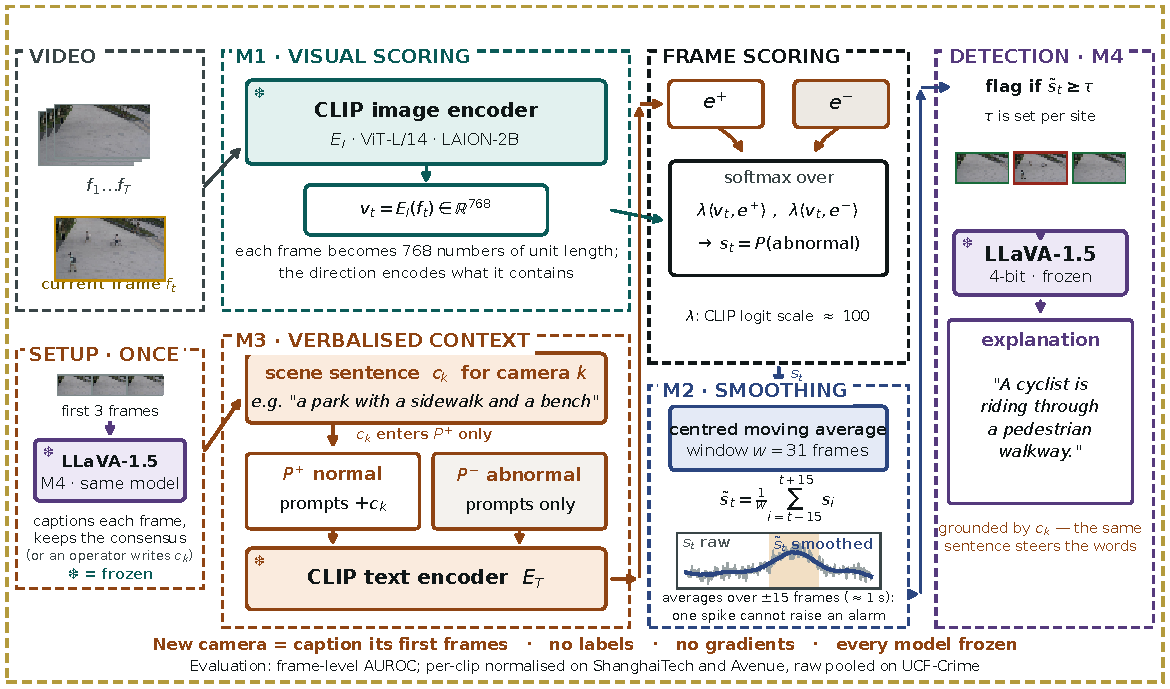
\includegraphics[width=0.97\textheight]{fig_architecture_clip}
\caption{The DA-ZVAD framework. Every model is frozen; the verbalised scene
context (M3) is the sole adaptation mechanism. At setup, the same frozen LLaVA
used for explanation captions a camera's first three frames, and the consensus
caption becomes that camera's descriptor $c_k$, so no human-written text is
required. $c_k$ enters the normal prompt ensemble only, and grounds the
generated explanations.}
\label{fig:arch}
\end{sidewaysfigure}

\begin{description}
  \item[M1 --- Visual encoder.] A frozen CLIP ViT-L/14 encoder
  \citep{radford2021clip} embeds each frame. The backbone is a Vision
  Transformer \citep{dosovitskiy2021vit}, built on the transformer architecture
  of \citet{vaswani2017attention}. It partitions the frame into
  $14 \times 14$ patches and produces one unit-norm embedding, placed in the
  joint image--text space that CLIP learns by contrastive pre-training. Scoring
  follows Equation~\eqref{eq:framescore}. No training data is used; the
  language prior serves as the classifier.

  \item[M2 --- Temporal aggregation.] Per-frame scores are smoothed by the
  centred moving average of Equation~\eqref{eq:smooth} over a window of $w$
  frames. This suppresses isolated single-frame fluctuations while preserving
  multi-frame events, and introduces no learnable parameters. The window width
  $w$ is the only hyperparameter of this stage and is swept in
  Section~\ref{sec:res-video}.

  \item[M3 --- Verbalised domain context.] A short natural-language description
  of the deployment scene is appended to the normal prompt ensemble only,
  grounding the notion of normality in the specific environment; one
  description is held per camera. This module is the adaptation
  mechanism of the framework. It is the vision-side counterpart of prompt-based
  adaptation as catalogued for language models by \citet{fan2026llm}, and
  differs from the verbalised learning of \citet{ye2025vera} in that the text is
  supplied at inference rather than optimised on source data beforehand.

  \item[M4 --- Reasoning and explanation.] A frozen multimodal large language
  model (LLaVA-1.5-7B \citep{liu2023llava}) serves two roles. At installation it
  captions the first frames of a camera's footage, and that caption becomes the
  camera's descriptor for M3, so that no human-written text is required. During
  operation, for each detected event, it receives the peak-scoring frame
  together with the descriptor and produces a natural-language explanation.
  The model is loaded under 4-bit
  \textsc{NormalFloat} quantisation \citep{dettmers2023qlora}, which reduces its
  memory footprint by roughly a factor of four relative to 16-bit weights, so
  that it fits beside the visual encoder on a single GPU. The effect of
  quantisation on caption and explanation quality has not been measured
  separately. The prompt explicitly permits the model to report that nothing
  appears wrong, which limits ungrounded assertions.
\end{description}

The complete pipeline is designed to fit a single consumer GPU, using
approximately 7\,GB of VRAM. This is a deliberate contrast to multi-model
training-free pipelines such as that of \citet{zanella2024lavad}, which chains a
captioner, a large language model and a cross-modal refiner.

\subsection{Inference algorithm}
Algorithm~\ref{alg:infer} gives the complete inference procedure for one video.
Lines~1--3 run once per camera, lines~4--8 once per sampled frame, and lines~9--13
once per detected event.

\begin{algorithm}[h]
\caption{DA-ZVAD inference for one sequence}
\label{alg:infer}
\begin{algorithmic}[1]
\Require frames $X = \{x_1,\dots,x_T\}$; domain descriptor $c$; window $w$;
         threshold $\tau$; frozen encoder $E$, frozen MLLM $G$
\Ensure per-frame scores $\tilde{s}$; event explanations $\mathcal{E}$
\State $(P^{+}, P^{-}) \gets \textproc{GroundPrompts}(c)$
       \Comment{M3: inject $c$ into prompt ensembles}
\State $e^{+} \gets \textproc{MeanPool}(E_{\text{text}}(P^{+}))$
\State $e^{-} \gets \textproc{MeanPool}(E_{\text{text}}(P^{-}))$
\For{$t = 1$ \textbf{to} $T$}
    \State $v_t \gets E_{\text{img}}(x_t)$ \Comment{M1: frozen visual embedding}
    \State $s_t \gets \textproc{Softmax}\!\left(\left[\langle v_t, e^{+}\rangle,\;
           \langle v_t, e^{-}\rangle\right]\cdot\lambda\right)_{2}$
           \Comment{$\lambda$: CLIP logit scale}
\EndFor
\State $\tilde{s} \gets \textproc{MovingAverage}(s, w)$ \Comment{M2}
\State $\mathcal{P} \gets \{t : \tilde{s}_t \ge \tau\}$
\State $\mathcal{V} \gets \textproc{PeakOfEachRun}(\mathcal{P}, \tilde{s})$
       \Comment{one explanation per event}
\ForAll{$t \in \mathcal{V}$}
    \State $\mathcal{E}[t] \gets G(x_t,\, c,\, \tilde{s}_t)$ \Comment{M4}
\EndFor
\State \Return $\tilde{s}, \mathcal{E}$
\end{algorithmic}
\end{algorithm}

\subsection{The context sweep protocol}
\label{sec:sweep}
To isolate the contribution of the domain descriptor, the pipeline is executed
repeatedly on identical data with every component fixed, varying only $c$ across
the four conditions of Table~\ref{tbl:variants}.

\begin{table}[width=\linewidth,cols=3,pos=htbp]
\caption{The four conditions of the context sweep. All models, frames,
thresholds and windows are held fixed; only the text differs.}
\label{tbl:variants}
\begin{tabularx}{\linewidth}{@{}l Z Z@{}}
\toprule
\textbf{Condition} & \textbf{Descriptor supplied} & \textbf{Purpose} \\
\midrule
none       & M3 disabled; prompt ensembles only & Lower reference \\
generic    & ``a generic scene''                & Controls for the mere presence of context \\
matched    & Correct description of the scene   & The proposed operating condition \\
mismatched & Description of the \emph{wrong} domain family (industrial text on surveillance data, and conversely) & \textbf{Falsifying control} \\
\bottomrule
\end{tabularx}
\end{table}

The predicted signature, if the adaptation claim holds, is
matched~$\gtrsim$~generic~$\gtrsim$~none, with mismatched performing measurably
\emph{worse}. The mismatched condition is essential: a method that ignores its
context entirely would show no difference across conditions, and a result of that
form would refute the claim rather than support it.

\subsection{Implementation}
The framework is implemented as a configuration-driven Python package in which
each module is independently switchable, so that the full ablation is produced by
configuration rather than by code modification. Experiments are cached and
resumable. The implementation has been verified end-to-end on synthetic data; the
measured results reported below are those obtained on real data.

Video experiments were run on a single NVIDIA A40 under PyTorch 2.3.1 with CUDA
12.1, using CLIP ViT-L/14 pretrained on LAION-2B. Each run records a manifest. It captures the
commit identifier of the code, the hardware, the library versions, the full
configuration, and the per-dataset sequence, frame and positive-label counts.
Every reported figure is therefore traceable to the state that produced it. Image embeddings are cached separately from scores: the visual encoder is
the only expensive stage and is independent of the prompts, the scoring rule and
the temporal window, so a single encoding pass supports the comparison of many
scoring hypotheses without re-encoding.

% =====================================================================
\section{Experimental Setup}
\label{sec:setup}
% =====================================================================

\subsection{Datasets}
Table~\ref{tbl:datasets} lists the six benchmarks and Fig.~\ref{fig:samples}
shows frames from two of them. MVTec~AD serves only as an image-level detection
baseline. For every video benchmark only the official test split is used; no
training video is used anywhere, since nothing is trained. Frames are sampled
every second frame on ShanghaiTech and CUHK Avenue (20{,}449 and 7{,}669 sampled
frames) and every sixteenth frame on UCF-Crime, XD-Violence and NWPU Campus
(69{,}634, 145{,}649 and 24{,}132), the latter matching the 16-frame snippets in
which XD-Violence is labelled and LAVAD's sampling on UCF-Crime
\citep{zanella2024lavad}.

\begin{table}[width=\linewidth,cols=3,pos=htbp]
\caption{Datasets. MVTec~AD is a detection baseline; the adaptation experiments
run on the video benchmarks, which span one scene (Avenue), twelve
(ShanghaiTech), 43 (NWPU Campus) and several hundred (UCF-Crime, XD-Violence).
XD-Violence and NWPU Campus are used in Section~\ref{sec:res-xd} to locate where
the method fails.}\label{tbl:datasets}
\begin{tabularx}{\linewidth}{@{}l l Z@{}}
\toprule
\textbf{Dataset} & \textbf{Domain} & \textbf{Content} \\
\midrule
MVTec AD \citep{bergmann2019mvtec} & Industrial & 15 product categories, 1{,}725 test images, pixel-level masks \\
ShanghaiTech \citep{liu2018shanghaitech} & Surveillance & Campus CCTV, 13 scenes (12 present in the test split), 107 test clips, 40{,}791 frames, frame-level ground truth \\
CUHK Avenue \citep{lu2013avenue} & Surveillance & Outdoor campus walkway, single view, 21 test videos, 15{,}324 frames \\
UCF-Crime \citep{sultani2018ucfcrime} & Surveillance & Real-world CCTV, 13 crime classes, test split of 290 videos (140 anomalous, 150 normal), frame-level temporal annotation \\
XD-Violence \citep{wu2020xdviolence} & Mixed video & Films, sports, games, news, CCTV and hand-held footage; six violence classes; test split of 800 videos (500 violent, 300 not); scored by average precision \\
NWPU Campus \citep{cao2023nwpu} & Surveillance & Campus CCTV, 43 scenes, 28 anomaly classes including scene-dependent ones; 242 test videos (124 with anomalies) \\
\bottomrule
\end{tabularx}
\end{table}

\begin{figure}[pos=htbp]
\centering
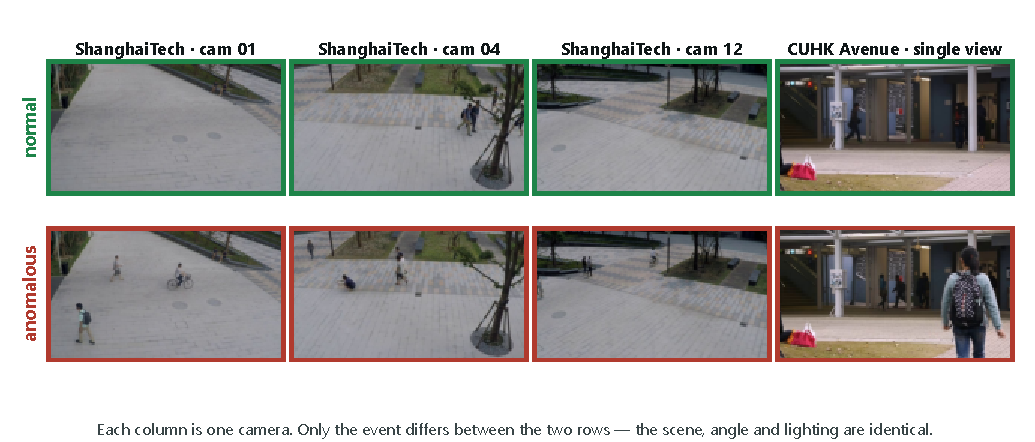
\includegraphics[width=\linewidth]{fig_dataset_samples}
\caption{Normal and anomalous frames from the two video benchmarks. Each column
is a single fixed camera, so within a column the scene, viewpoint and lighting
are constant and only the event differs. The label is therefore a property of
what is happening rather than of how the scene appears---an empty walkway and
the same walkway carrying a cyclist are visually similar and oppositely
labelled, which is the concept shift of Section~\ref{sec:gap} in a
photograph.}\label{fig:samples}
\end{figure}

\subsection{Evaluation metrics}
\label{sec:metrics}
Anomaly detection is strongly class-imbalanced, so accuracy is uninformative: a
detector that labels every frame normal attains high accuracy while detecting
nothing. Every measure used here is therefore threshold-free and is computed
directly from the detector's output $\tilde{s}$ (Table~\ref{tbl:io}). Let
$\mathcal{A}$ be the set of anomalous evaluation frames and $\mathcal{N}$ the set
of normal ones, each frame $i$ carrying score $\tilde{s}_i$ and label
$y_i \in \{0,1\}$.

\emph{Frame-level AUROC (primary).} The area under the receiver operating
characteristic curve \citep{fawcett2006roc, bradley1997auc}, which traces the
true-positive rate $\mathrm{TPR}(\tau)=|\{i\in\mathcal{A}:\tilde{s}_i\ge\tau\}|/|\mathcal{A}|$
against the false-positive rate
$\mathrm{FPR}(\tau)=|\{i\in\mathcal{N}:\tilde{s}_i\ge\tau\}|/|\mathcal{N}|$ as the
threshold $\tau$ falls. It equals the probability that a randomly chosen
anomalous frame scores above a randomly chosen normal one,
\begin{equation}
\mathrm{AUROC} \;=\; \frac{1}{|\mathcal{A}|\,|\mathcal{N}|}
\sum_{i\in\mathcal{A}}\sum_{j\in\mathcal{N}}
\Big(\mathbf{1}[\tilde{s}_i>\tilde{s}_j] + \tfrac{1}{2}\,\mathbf{1}[\tilde{s}_i=\tilde{s}_j]\Big),
\label{eq:auroc}
\end{equation}
so $0.5$ is chance and $1$ is a perfect ranking. Because it depends only on the
ranking, it compares methods that calibrate their scores differently. It is
reported at image level on MVTec~AD and at frame level on video, following each
benchmark \citep{bergmann2019mvtec, liu2018shanghaitech}; pixel-level AUROC
against the defect masks is reported for localisation on MVTec~AD.

\emph{Micro and macro averaging.} The micro figure pools the frames of all videos
into one ranking before applying Equation~\eqref{eq:auroc}; this is the
convention on every benchmark used here, and it is the figure reported unless
stated otherwise. The macro figure applies Equation~\eqref{eq:auroc} within each
video and averages over videos. Pooled ranking compares frames from different
cameras against one another, so it is sensitive to each camera's score level,
whereas the macro figure is not; the measurement audit
(Section~\ref{sec:res-audit}) uses exactly this difference.

\emph{Per-clip normalisation.} On ShanghaiTech and CUHK Avenue each clip's
scores are min--max normalised,
$\hat{s}_t = (\tilde{s}_t-\min_k \tilde{s}_k)/(\max_k \tilde{s}_k-\min_k \tilde{s}_k)$,
before pooling, following the protocol established with the benchmark
\citep{liu2018shanghaitech}. The step uses no labels. On UCF-Crime, XD-Violence
and NWPU Campus scores are pooled raw: half of their test videos contain no
anomaly, and normalising such a video forces some of its frames to the maximum
score. Raw and normalised figures are reported side by side where both are
informative (Table~\ref{tbl:video}).

\emph{Average precision on XD-Violence (primary there).} XD-Violence defines
frame-level average precision as its metric, because AUROC ``usually shows an
optimistic result when dealing with class-imbalanced data''
\citep{wu2020xdviolence}. With precision
$\mathrm{P}(\tau)=|\{i\in\mathcal{A}:\tilde{s}_i\ge\tau\}|/|\{i:\tilde{s}_i\ge\tau\}|$
and recall $\mathrm{R}(\tau)=\mathrm{TPR}(\tau)$,
\begin{equation}
\mathrm{AP} \;=\; \int_{0}^{1} \mathrm{P}\,\mathrm{d}\mathrm{R},
\label{eq:ap}
\end{equation}
computed as the official code does, by the trapezoidal rule over the
precision--recall curve with each 16-frame snippet's score assigned to its
frames. The step-wise (non-interpolated) estimate agrees with it to within
$0.0001$ on our scores, so the figure is not inflated by ties
\citep{song2026vlmanswer}. AP rewards ranking the minority class correctly more
strongly than AUROC does \citep{davis2006pr}.

\emph{The context gap.} The quantity the context sweep exists to measure is the
difference in the metric between two descriptions supplied to the same frozen
pipeline,
\begin{equation}
\Delta(c_1, c_2) \;=\; \mathrm{M}\big(\tilde{s}(\cdot \mid c_1)\big) -
\mathrm{M}\big(\tilde{s}(\cdot \mid c_2)\big),
\label{eq:gap}
\end{equation}
where $\mathrm{M}$ is AUROC or AP. The headline gap is
$\Delta(\text{matched},\text{mismatched})$; because no parameter differs between
the two runs, $\Delta$ is attributable to the text (Section~\ref{sec:problem}).

\emph{Uncertainty.} Frames within a video are strongly correlated, so
uncertainty is estimated by resampling whole videos. For a gap $\Delta$, the $n$
test videos are drawn with replacement $B=1000$ times with a fixed seed, both
conditions are scored on the same draw, and the 95\% interval is the 2.5th to
97.5th percentile of the $B$ resampled gaps. A difference is called significant
when that interval excludes zero. This is done for UCF-Crime, XD-Violence and
NWPU Campus; on ShanghaiTech, where configurations were also selected, the spread
over five clip-level development/held-out partitions is reported instead
(Section~\ref{sec:res-components}).

% =====================================================================
\section{Results}
\label{sec:results}
% =====================================================================

\subsection{A detection baseline on MVTec AD}
\label{sec:res-mvtec}
The frozen visual scoring stage (M1) was evaluated on the complete MVTec~AD
benchmark \citep{bergmann2019mvtec} with no training data of any kind. As a
\emph{trained} reference we fit a One-Class Support Vector Machine
\citep{scholkopf2001oneclass}---which estimates the support of the normal-class
distribution and flags points falling outside it---on CLIP features of the
normal training split, using an RBF kernel after per-dimension standardisation.
The baseline consumes identical features and is evaluated on the identical test
split. The only difference between the two rows of Table~\ref{tbl:mvtec} is
therefore whether training on normal data took place, and the comparison
isolates the value of that training.

\begin{table}[width=\linewidth,cols=4,pos=htbp]
\caption{MVTec AD, 15 categories, 1{,}725 test images. CLIP ViT-L/14. Best
$F_1 = 90.7\%$.}\label{tbl:mvtec}
\begin{tabularx}{\linewidth}{@{}Z l l l@{}}
\toprule
\textbf{Method} & \textbf{Training data} & \textbf{Image AUROC} & \textbf{Pixel AUROC} \\
\midrule
One-Class SVM (CLIP features) & Normal images only & 92.4\% & --- \\
\textbf{DA-ZVAD M1 (zero-shot)} & \textbf{None} & \textbf{88.5\%} & \textbf{71.0\%} \\
\bottomrule
\end{tabularx}
\end{table}

A detector using no training data lands within roughly four points of a trained
baseline built on identical features. The per-category breakdown is more
informative than the mean. Performance separates sharply into two groups:
texture categories (carpet, grid, leather, tile, wood) average $\approx 99.5\%$,
while object categories (bottle, cable, capsule, transistor and others) average
$\approx 83.1\%$.
Zero-shot scoring \emph{exceeds} the trained baseline on every texture category
and on \texttt{screw} (84.3\% against 67.3\%), while the trained baseline retains
an advantage on structured objects with small, spatially localised defects
(transistor: 72.7\%).

The interpretation is that whole-image embeddings capture global appearance
changes, which the language prior describes well, but cannot resolve defects
occupying a small fraction of the pixels. A prompt-design ablation (generic
single prompt 89.1\%; category-specific single prompt 88.6\%; category-specific
ensemble 88.5\%) shows that prompt engineering yields no improvement at image
level, indicating that the binding constraint is spatial resolution rather than
linguistic specification. This finding motivates the windowed scoring used for
localisation and, more broadly, supports the position that the residual
difficulty for a foundation model in this task is not covariate in nature.

\subsection{Video detection without a description}
\label{sec:res-video}
ShanghaiTech was evaluated in full: all 107 test clips, 20{,}449 frames after
subsampling at $\mathrm{step}=2$, of which 8{,}671 ($42.4\%$) are anomalous.
Table~\ref{tbl:video} reports the M1$+$M2 configuration---frozen CLIP scoring
with moving-average aggregation, no domain descriptor---under all three pooling
conventions.

\begin{table}[width=\linewidth,cols=6,pos=htbp]
\caption{ShanghaiTech, 107 clips / 20{,}449 frames. Frame-level AUROC by
temporal window $w$, under three pooling conventions. Rows differ only in how
per-clip scores are aggregated into a single figure; the underlying scores are
identical.}\label{tbl:video}
\begin{tabularx}{\linewidth}{@{}Z l l l l l@{}}
\toprule
\textbf{Pooling convention} & $w{=}1$ & $w{=}5$ & $w{=}9$ & $w{=}15$ & $w{=}31$ \\
\midrule
Micro, raw scores            & 0.493 & 0.502 & 0.508 & 0.513 & 0.519 \\
Macro (per-clip mean)        & 0.614 & 0.628 & 0.637 & 0.648 & 0.670 \\
\textbf{Micro, per-clip normalised} & \textbf{0.667} & \textbf{0.685} & \textbf{0.691} & \textbf{0.702} & \textbf{0.707} \\
\bottomrule
\end{tabularx}
\end{table}

Two findings follow. First, temporal aggregation contributes a consistent gain
of four AUROC points from $w{=}1$ to $w{=}31$, present in every row and in every
context condition measured subsequently. The gain is bounded rather than
monotone: performance peaks at $w{=}31$ and falls back to $0.683$ at $w{=}61$,
so the window has a genuine optimum and the metric is not simply rewarding
heavier smoothing. M2 requires no training and no parameters, so the gain is
obtained at zero cost.

Second, and more consequential for evaluation practice, the raw micro figure is
indistinguishable from chance while the same scores yield $0.707$ once
normalised per clip. The gap is diagnostic rather than cosmetic. ShanghaiTech
spans twelve camera views, and a frozen scorer sits at a different similarity
baseline under each; concatenating raw scores therefore ranks frames drawn from
incomparable scales against one another, destroying an ordering that is present
within each clip. That the macro figure---which is by construction immune to
cross-clip offsets---sits at $0.670$ while raw micro sits at $0.519$ confirms
the cause. Only $31$ of $105$ scorable clips fall below chance individually.

Figure~\ref{fig:baselines} shows the cause directly. Frame embeddings projected
to two dimensions separate cleanly by camera, and each camera's similarity to
the global mean sits at its own level---from $0.77$ on view~06 to $0.91$ on
view~10. A raw score of a given magnitude therefore carries different evidence
under different cameras, and concatenating them compares quantities that were
never on a common scale.

\begin{figure}[pos=htbp]
\centering
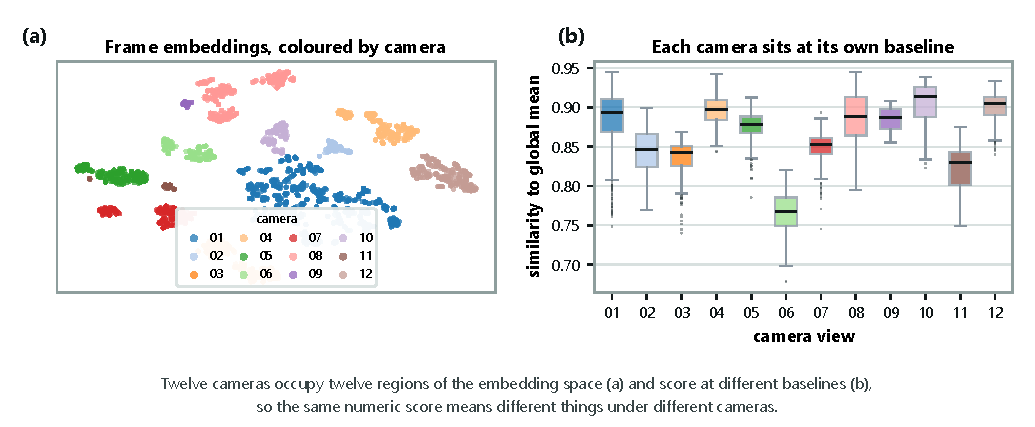
\includegraphics[width=\linewidth]{fig_camera_baselines}
\caption{Why pooling raw scores across cameras fails. (a) Frame embeddings
projected with t-SNE, coloured by camera view: the views occupy distinct
regions. (b) Distribution, per view, of each frame's similarity to the global
mean embedding; the medians differ by more than $0.13$. Neither panel uses
labels.}\label{fig:baselines}
\end{figure}

This is a concrete instance of the paper's general position appearing inside the
measurement itself: what counts as an anomalous \emph{score} is scene-relative,
exactly as what counts as an anomalous \emph{event} is.

\begin{figure}[pos=htbp]
\centering
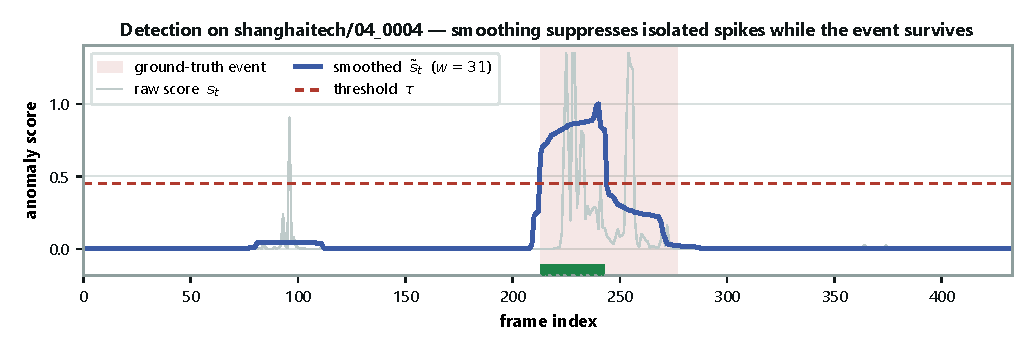
\includegraphics[width=\linewidth]{fig_detection_example}
\caption{One clip scored end to end. The raw per-frame score is noisy enough
that isolated frames outside the event exceed the level reached inside it;
the moving average of Equation~\eqref{eq:smooth} suppresses those excursions
while the event, which persists across many frames, survives. This is the
mechanism behind the monotone gains of Table~\ref{tbl:video}.}\label{fig:detect}
\end{figure}

\subsection{The context sweep}
\label{sec:res-sweep}
The sweep of Section~\ref{sec:sweep} was run twice, differing only in how the
domain descriptor is fused into the prompt ensembles. In the \emph{both}
condition the descriptor is appended to the normal and the abnormal ensemble
alike; in the \emph{normal} condition it is appended only to the normal
ensemble. Every other quantity---weights, prompts, data, protocol---is
identical, and in Table~\ref{tbl:sweep} the \texttt{none} column is common to
both rows by construction, which serves as an internal control.
Figure~\ref{fig:chartsweep} plots the same numbers with the matched--mismatched
distance drawn explicitly for each fusion rule.

\begin{table}[width=\linewidth,cols=6,pos=htbp]
\caption{Context sweep on ShanghaiTech at the optimal window $w{=}31$, per-clip
normalised frame-level AUROC over all 107 clips. All models frozen; only the
domain descriptor and its point of injection vary. The \texttt{none} column is
necessarily identical across rows and confirms that no other quantity
changed.}\label{tbl:sweep}
\begin{tabularx}{\linewidth}{@{}Z l l l l l@{}}
\toprule
\textbf{Fusion} & \textbf{none} & \textbf{generic} & \textbf{matched} & \textbf{mismatched} & \textbf{gap} \\
\midrule
Both ensembles          & 0.707 & 0.670 & 0.666 & 0.695 & $-0.029$ \\
\textbf{Normal ensemble only} & \textbf{0.707} & \textbf{0.691} & \textbf{0.734} & \textbf{0.628} & $\mathbf{+0.105}$ \\
\bottomrule
\end{tabularx}
\end{table}

\begin{figure}[pos=htbp]
\centering
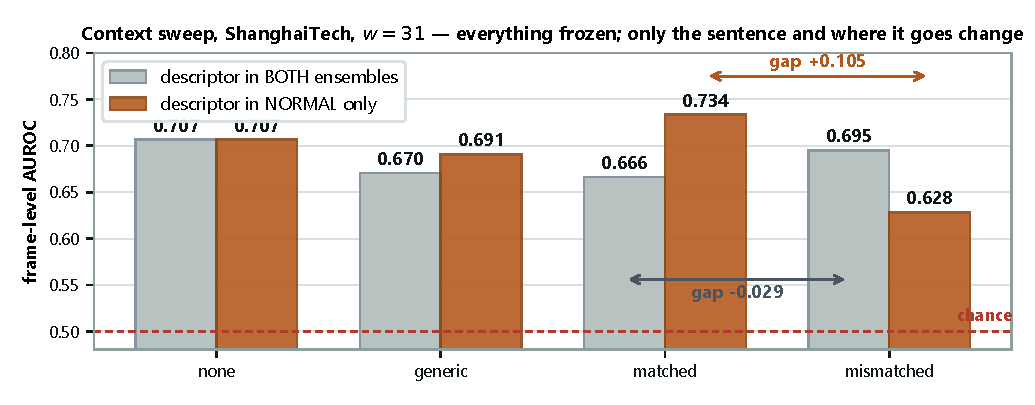
\includegraphics[width=\linewidth]{fig_chart_sweep}
\caption{Table~\ref{tbl:sweep} drawn. The quantity the sweep exists to produce is
the distance between the matched and mismatched bars, which is annotated for
each fusion rule. Moving the descriptor from both ensembles to the normal
ensemble alone changes that distance from $-0.029$ to
$+0.105$.}\label{fig:chartsweep}
\end{figure}

Under \emph{both}, the predicted ordering is not merely absent but reversed: the
matched descriptor is the \emph{worst} condition ($0.666$) and the deliberately
mismatched one among the best ($0.695$). The mechanism is prototype dilution.
Each ensemble is mean-pooled into a single embedding. Text appended to both
ensembles therefore enters both prototypes as a common component, which draws
them together and contracts the margin that carries the decision.

The collapse is directly measurable, since the prototypes are mean-pooled text
embeddings and the angle between them requires no images. Table~\ref{tbl:proto}
reports it.

\begin{table}[width=\linewidth,cols=5,pos=htbp]
\caption{Angle between the normal and abnormal prototypes under each condition,
with the margin $1-\cos$ and the corresponding AUROC. The prototypes are
mean-pooled text embeddings, so this is a property of the prompts alone.}
\label{tbl:proto}
\begin{tabularx}{\linewidth}{@{}Z l l l l@{}}
\toprule
\textbf{Fusion} & \textbf{none} & \textbf{generic} & \textbf{matched} & \textbf{mismatched} \\
\midrule
Both ensembles  & $35.7^\circ$ & $26.3^\circ$ & $26.3^\circ$ & $25.0^\circ$ \\
Normal only     & $35.7^\circ$ & $34.5^\circ$ & $\mathbf{41.9^\circ}$ & $37.6^\circ$ \\
\bottomrule
\end{tabularx}
\end{table}

Two things follow, and they do not both favour the account.

The collapse is real and large. Injecting a descriptor into both ensembles
contracts the prototype angle from $35.7^\circ$ to between $25^\circ$ and
$26^\circ$, nearly halving the margin, and it does so for every descriptor
tested. Injecting into the normal ensemble alone produces no such contraction;
the matched descriptor instead \emph{widens} the angle to $41.9^\circ$, above
the ungrounded baseline, and that condition also attains the highest AUROC. The
fusion rule therefore behaves geometrically as the account claims.

The finer ordering does not follow the geometry. We anticipated that an accurate
descriptor would collapse the prototypes furthest, since accurate text aligns
with every frame; in fact the mismatched descriptor collapses them marginally
more ($0.907$ against $0.895$ cosine), and the three grounded conditions sit
within $1.3^\circ$ of one another while their AUROC spans $0.029$. Prototype
separation thus explains why grounding both ensembles is harmful, but not why an
accurate descriptor is the most harmful of the three.

What the angle cannot see is the \emph{direction} of the collapse. Two
prototypes can close by the same amount while moving toward the region the
image embeddings occupy or away from it, and the two cases predict opposite
things: a pair drawn onto the images makes every frame score alike, whereas a
pair drawn elsewhere leaves the original prompts discriminating underneath. We
measured this directly, as the mean cosine similarity between the image
embeddings and the two prototypes, on a sample of $2{,}675$ ShanghaiTech frames
spanning all twelve views (Table~\ref{tbl:direction}). The prompts and pooling
used reproduce all eight angles of Table~\ref{tbl:proto} exactly, and the sample
reproduces the published ordering of conditions under both fusion rules.

\begin{table}[width=\linewidth,cols=4,pos=htbp]
\caption{Direction of the prototype collapse under \emph{both} fusion: mean
cosine similarity between the frame embeddings and each prototype, and the
movement of the pair relative to \texttt{none}. Prototype angles are those of
Table~\ref{tbl:proto}.}\label{tbl:direction}
\begin{tabularx}{\linewidth}{@{}Z l l l@{}}
\toprule
\textbf{Condition} & \textbf{Angle} & \textbf{Pair to images} & \textbf{Change} \\
\midrule
none       & $35.7^\circ$ & 0.216 & --- \\
generic    & $26.3^\circ$ & 0.230 & $+0.014$ \\
\textbf{matched}    & $26.3^\circ$ & \textbf{0.282} & $\mathbf{+0.067}$ \\
mismatched & $25.0^\circ$ & 0.199 & $-0.017$ \\
\bottomrule
\end{tabularx}
\end{table}

The accurate descriptor collapses the prototypes by no more than the others but
drags the pair onto the images almost five times as far as the placeholder does,
while the mismatched descriptor moves it the opposite way. That is the ordering
the AUROC shows---matched worst, mismatched close to \texttt{none}---and it
completes the account: grounding both ensembles is harmful because it contracts
the margin, and an accurate description is the \emph{most} harmful because it
also places both prototypes where the frames are. A second candidate, the
per-frame spread of the margin, does not follow the ordering (matched $0.0138$
against mismatched $0.0133$) and is not the operative quantity.

Under \emph{normal}, where the descriptor no longer enters both prototypes, the
predicted signature appears: matched $(0.734) >$ none $(0.707) \gg$ mismatched
$(0.628)$. The matched-minus-mismatched contrast moves from $-0.029$ to
$+0.105$; fixing the fusion rule inverts the sign of the effect.

The two halves of that signature carry different evidential weight, and the
distinction should be stated rather than blurred. The matched-over-none margin
is $+0.027$. It is positive at every window measured and grows with the window
($+0.008$, $+0.007$, $+0.010$, $+0.012$, $+0.027$, $+0.038$ at $w = 1, 5, 9, 15,
31, 61$), which is a consistent direction rather than a chance ordering. It
nonetheless lies inside the split-to-split spread of $\pm 0.036$ reported in
Section~\ref{sec:res-components}, so we report the direction and decline to
claim the magnitude.

The mismatched deficit is $-0.105$ and is unambiguous. What the experiment
establishes is therefore that the descriptor is \emph{load-bearing}: corrupting
it degrades detection substantially, whether or not supplying the correct one
measurably improves on supplying none. Because no parameter is updated anywhere
in the pipeline, that deficit is attributable to the text alone---no other
quantity was free to vary. This is the identifiability property of
Section~\ref{sec:problem} realised as a measurement.

Figure~\ref{fig:ctxeffect} shows the effect on a single clip rather than as a
summary statistic. The two curves come from the same frozen models scoring the
same frames; only the descriptor differs. They track each other outside the
event and separate within it, which is what the aggregate gap of $+0.105$
measures one clip at a time.

\begin{figure}[pos=htbp]
\centering
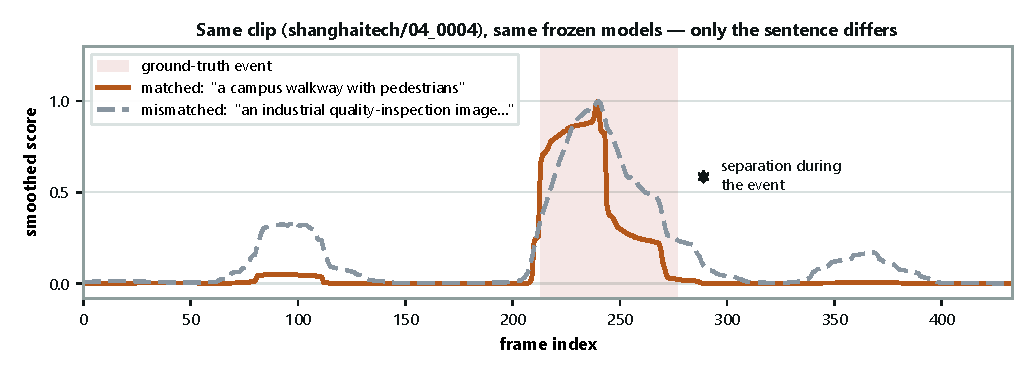
\includegraphics[width=\linewidth]{fig_context_effect}
\caption{The descriptor's contribution, per frame. Identical models, identical
frames, identical smoothing; the only difference is whether the supplied
sentence describes the scene or an industrial site. Because no parameter is free
to vary, the separation between the curves is attributable to the text
alone.}\label{fig:ctxeffect}
\end{figure}

A secondary consequence is methodological. Verbalised context is frequently
treated as a matter of wording; here the point of injection dominated the
wording entirely, to the extent of reversing the direction of the effect. A
negative result reported without varying the fusion rule would have been an
artefact of an implementation detail.

\subsection{Ablation study}
\label{sec:res-components}
To establish what each signal contributes, image embeddings were cached once and
five scoring rules compared against them. Two are semantic (a text margin
against the prompt ensembles); one is kinematic (embedding drift between
neighbouring frames of a clip, requiring no additional model); one estimates
normality from the clip's own unlabelled frames; and two combine them by
per-clip standardisation.

Because cached embeddings make evaluation nearly free, the risk of selecting a
configuration that succeeds by chance is real. Clips were therefore partitioned
into development and held-out halves before measurement, at the clip level
rather than the frame level---frames within a clip are strongly correlated, so a
frame-level partition would leak across the boundary. Five independent
partitions were drawn; ranking used the development halves only.
Table~\ref{tbl:components} reports the outcome, and
Figure~\ref{fig:chartablation} places it beside the window sweep that fixed
$w{=}31$.

\begin{table}[width=\linewidth,cols=4,pos=htbp]
\caption{Component ablation on ShanghaiTech. Held-out AUROC is the mean over
five clip-level partitions, with the standard deviation across
partitions; the final column scores every clip, for comparability with published
results that use the full test set.}\label{tbl:components}
\begin{tabularx}{\linewidth}{@{}Z l l l@{}}
\toprule
\textbf{Scoring signal} & $w$ & \textbf{Held-out} & \textbf{Full set} \\
\midrule
Scene-centre normality only      & 31 & $0.585 \pm 0.025$ & 0.585 \\
Semantic $+$ scene-centre        & 31 & $0.645 \pm 0.034$ & 0.640 \\
Kinematic (embedding drift) only & 31 & $0.685 \pm 0.015$ & 0.686 \\
Semantic $+$ kinematic           & 31 & $0.711 \pm 0.034$ & 0.706 \\
\textbf{Semantic (text margin) only} & 31 & $\mathbf{0.718 \pm 0.036}$ & \textbf{0.707} \\
\bottomrule
\end{tabularx}
\end{table}

\begin{figure*}[pos=htbp]
\centering
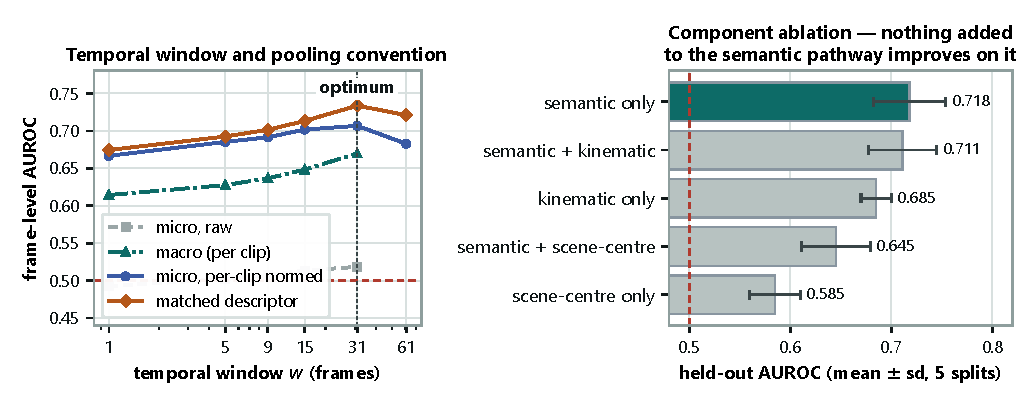
\includegraphics[width=\linewidth]{fig_chart_ablation}
\caption{Left: frame-level AUROC against the temporal window $w$ under each
pooling convention, with the matched-descriptor curve for comparison. Raw
micro-pooling never leaves chance at any window, and every curve turns down
after $w{=}31$. Right: Table~\ref{tbl:components} drawn, held-out mean with the
standard deviation across the five partitions. The intervals of the top three
configurations overlap, so the claim the panel supports is that nothing added to
the semantic pathway improves on it---not that semantic-only is separated from
the alternatives.}\label{fig:chartablation}
\end{figure*}

The semantic signal alone is the strongest configuration, and nothing added to
it helps. Combining it with the kinematic signal costs $0.001$ on the full test
set and $0.007$ on held-out clips; combining it with scene-centre normality
costs $0.067$. The kinematic signal is worthwhile only in isolation, where it
reaches $0.686$ without consulting language at all, but it is not additive with
the pathway that does.

This is a negative result about the framework's own elaborations rather than
about the benchmark. The natural reading of ShanghaiTech's anomaly classes is
that they require two conditions jointly---a stationary bicycle is not anomalous,
nor is a pedestrian walking briskly, whereas a bicycle \emph{travelling at
cycling speed} on a walkway is---which predicts that appearance and motion
should be complementary. They are not, at least as measured here. The frozen
encoder's pooled embedding evidently already registers enough of the motion for
an explicit kinematic term to add nothing.

Six modifications were tested against the plain semantic scorer and none
improved on it. They are recorded here rather than omitted, because a claim that
a minimal configuration is the right one is only credible alongside the
alternatives that were tried.

\begin{enumerate}[(i)]
  \item \emph{Scene-centre normality}, in which the mean embedding of a clip's
        own frames defines normality and departure from it defines anomaly,
        reaches $0.585$ and degrades the semantic signal when combined with it.
  \item \emph{Kinematic scoring} adds nothing to the semantic pathway, as above.
  \item \emph{Local temporal deviation}, which subtracts a windowed reference
        before projecting onto the text direction, reaches $0.686$ alone and
        also narrows the context gap of Section~\ref{sec:res-sweep} to below
        $0.02$---it improves the scorer at the cost of the effect being measured.
  \item \emph{Quadrant-level scoring}, intended to recover anomalies too small
        to survive the $224\times224$ resize, did not improve on whole-frame
        scoring in any configuration. Mean aggregation over quadrants beat
        maximum aggregation, which is the reverse of what recovering a small
        object would produce and is consistent instead with mild ensembling.
  \item \emph{Per-prompt maximum pooling} in place of mean-pooled prototypes
        scores $0.678$ against $0.707$.
  \item \emph{A domain-specific prompt ensemble} naming ShanghaiTech's
        documented anomaly classes reaches $0.486$ against $0.685$ for the
        generic surveillance ensemble at $w{=}5$. This follows from the dilution
        mechanism of Section~\ref{sec:res-sweep}: its normal and abnormal
        prompts share heavy scene vocabulary---``walkway'',
        ``pedestrians''---which contracts the margin between prototypes in
        exactly the manner the fusion experiment isolated.
\end{enumerate}

Region-level scoring at finer granularity than quadrants remains untested and is
identified in Section~\ref{sec:conclusion} as the most promising route to a
materially higher figure.

\subsection{A single-camera benchmark and the within-view control}
\label{sec:res-avenue}
The identical frozen configuration was applied to CUHK Avenue
\citep{lu2013avenue}: 21 test clips, 7{,}669 frames after subsampling, of which
$24.2\%$ are anomalous. Nothing was retuned. Only the scene descriptor was
changed, from a campus walkway to an outdoor walkway before a building entrance,
which is what the framework claims is sufficient to redeploy it.

\begin{table}[width=\linewidth,cols=6,pos=htbp]
\caption{The context sweep on three of the video benchmarks, one shared
descriptor per benchmark, normal-ensemble fusion, frame-level AUROC. The
configuration is identical; only the dataset and the scene descriptor differ.
ShanghaiTech and Avenue: $w{=}31$, per-clip normalised. UCF-Crime: $w{=}5$ (the
same duration at its sampling, Section~\ref{sec:res-ucf}), shown under both its
pre-registered primary metric (raw pooled) and the campus protocol (per-video
normalised); the two disagree on the size of the gap, and both are given.}
\label{tbl:avenue}
\begin{tabularx}{\linewidth}{@{}Z l l l l l@{}}
\toprule
\textbf{Dataset} & \textbf{none} & \textbf{generic} & \textbf{matched} & \textbf{mismatched} & \textbf{gap} \\
\midrule
ShanghaiTech & 0.707 & 0.691 & \textbf{0.734} & 0.628 & $+0.105$ \\
CUHK Avenue  & 0.706 & \textbf{0.729} & 0.677 & 0.657 & $+0.020$ \\
UCF-Crime, raw (primary)        & 0.756 & 0.729 & \textbf{0.813} & 0.727 & $+0.086$ \\
UCF-Crime, per-video normalised & 0.759 & 0.740 & \textbf{0.767} & 0.746 & $+0.021$ \\
\bottomrule
\end{tabularx}
\end{table}

Detection transfers. With no descriptor the two benchmarks give $0.706$ and
$0.707$, which is as close to identical as this measurement resolves. A frozen
encoder and a pair of prompt ensembles carry over between two surveillance
domains without adjustment, which is the covariate-shift half of the problem and
is consistent with Observation~3.

The adaptation mechanism does not transfer. The matched-minus-mismatched gap
falls from $+0.105$ to $+0.020$, and the matched descriptor now scores
\emph{below} supplying none. The best condition on Avenue is \texttt{generic}: a
placeholder reading ``a generic scene'' outperforms an accurate description of
the scene by $0.052$. Since \texttt{generic} carries no information about the
deployment environment, whatever benefit it confers cannot be domain adaptation;
the most economical reading is that an additional prompt improves the normal
ensemble as an ensemble, independently of what it says.

A residual effect survives. The mismatched condition remains the worst on both
benchmarks, so a description of the wrong domain still costs something even
where the correct one does not help. That the effect is directionally consistent
and an order of magnitude weaker is more informative than either a clean
replication or a flat null would have been.

We attribute the difference to scene diversity. The ShanghaiTech test split spans twelve
camera views, so a descriptor has a discrimination to perform: it states which
of several environments the model is operating in. Avenue is a single fixed
view, and every clip shows it, so there is nothing for a scene description to
resolve and the base prompts already cover the only environment present. This
predicts that the utility of verbalised context scales with the domain variation
it must resolve, and that a benchmark with one scene is close to the floor of
that scale. The floor is confirmed below; the proportional form was later
registered and tested on UCF-Crime and refuted (Section~\ref{sec:res-ucf}).

That account makes a prediction on ShanghaiTech alone, because ShanghaiTech is
twelve single-view datasets stacked together. Partitioning it by camera and
running the same sweep inside each view should reproduce Avenue's flat result,
while the pooled evaluation reproduces the effect. A within-view gap comparable
to the pooled one would refute the account outright.

\begin{table}[width=\linewidth,cols=4,pos=htbp]
\caption{The context gap (matched $-$ mismatched) against the number of scenes
the descriptor must resolve. ShanghaiTech rows: $w{=}31$, the sweep evaluated
inside each camera view separately and pooled. Of the twelve test views, the
three with fewer than four scorable clips or only one class present (02, 09,
11) are excluded.
The UCF-Crime row was added later and is the test of prediction~P1
(Section~\ref{sec:res-ucf}): per-video generated descriptors, raw pooled,
$w{=}5$.}\label{tbl:withinview}
\begin{tabularx}{\linewidth}{@{}Z l l l@{}}
\toprule
\textbf{Evaluation} & \textbf{Scenes} & \textbf{Clips} & \textbf{Gap} \\
\midrule
CUHK Avenue (single view)    & 1  & 21  & $+0.020$ \\
\textbf{ShanghaiTech, mean within a view}  & 1 each, 9 views  & 5--34 each & $\mathbf{+0.033}$ (sd $0.058$) \\
ShanghaiTech, pooled across views          & 12 & 107 & $+0.105$ \\
UCF-Crime, per-video descriptors & ${\sim}290$ & 290 & $+0.096$ \\
\bottomrule
\end{tabularx}
\end{table}

\begin{figure}[pos=htbp]
\centering
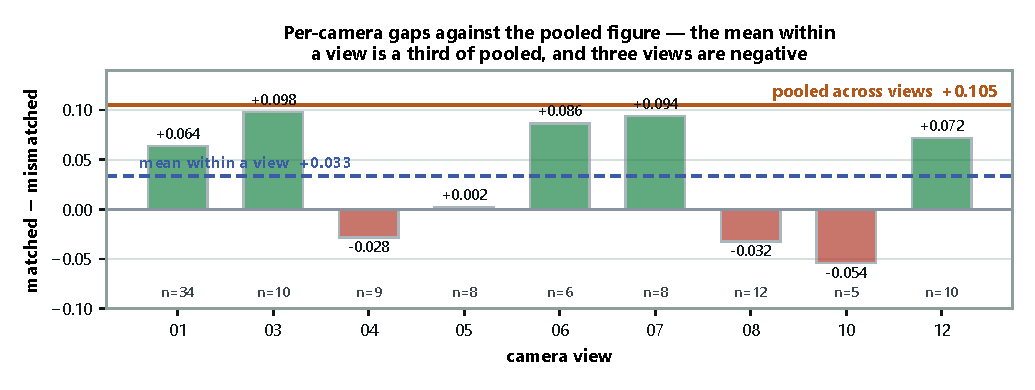
\includegraphics[width=\linewidth]{fig_chart_within_view}
\caption{The context gap measured inside each camera view separately, against the
pooled figure of Table~\ref{tbl:sweep}. Almost every view falls well short of the
pooled bar and three return negative gaps, but two views (03 and 07) approach it;
the finding is in the mean and the spread, not in a uniform collapse. Clip counts
per view are printed below the axis.}\label{fig:chartwithin}
\end{figure}

The prediction holds. Table~\ref{tbl:withinview} summarises it and
Figure~\ref{fig:chartwithin} shows the per-view detail behind the mean.
Confining the evaluation to a single environment reduces
the gap to roughly a third of its pooled value, placing it near the figure
measured on single-view Avenue. What the descriptor contributes is therefore
substantially the resolution of \emph{which} scene is in view, rather than a
characterisation of normality \emph{within} a scene.

Three qualifications attach to that conclusion. The within-view estimates are
noisy: each rests on between five and thirty-four clips, and three of the nine
views return negative gaps, so the effect is not reliably positive inside a
single view---which is the substance of the finding rather than a defect in it.
The reduction is partial, not total: a third of the effect survives within one
scene, so scene identification does not account for all of it. And the views
differ enormously in difficulty, from $0.911$ on view~05 to $0.415$ on view~12,
the latter below chance; a mean over such heterogeneous conditions should be
read as an indication rather than a precise quantity.

Those qualifications can be made quantitative, and doing so separates two claims
the mean alone blurs. Resampling the nine views $50{,}000$ times gives a 95\%
percentile interval of $[-0.005, +0.070]$ on the within-view gap. The claim this
section makes---that confining the evaluation to one view \emph{shrinks} the
gap---is established: the interval excludes the pooled $+0.105$, and no
resample reaches it. The stronger claim, that the within-view gap is above zero,
is not: the interval includes zero. The negative views are not an artefact of
small views (the correlation between gap and clip count is $+0.19$), and
Avenue's $+0.020$ lies inside the interval, so the single-camera benchmark is
statistically indistinguishable from a single ShanghaiTech view rather than
merely close to one. The standard deviation printed in
Table~\ref{tbl:withinview} is the population figure; the sample standard
deviation over the nine views is $0.061$.

\subsection{A description per camera, written by hand and by the model}
\label{sec:res-perview}
If the descriptor's contribution is to identify which scene is in view, a single
sentence shared by all twelve ShanghaiTech views is the wrong unit: it cannot
tell the views apart. The account predicts that a sentence written for each view
should do better, and that the gain should vanish if each view is given another
view's sentence. The second condition is the control that matters. Every
sentence in it is a plausible description of a campus scene, so a model that
merely rejected implausible text---which the industrial \texttt{mismatched}
condition cannot rule out---would score it as well as the correct assignment.

Two sets of per-view sentences were scored. The first was written by hand from
one normal frame per view, once, with no revision. The second was generated
without human input by the framework's own reasoning model (M4, LLaVA-1.5-7B,
frozen and 4-bit), captioning the first three frames of each view's first clip
under an instruction to describe the place and not the people, and keeping the
caption closest to the other two in the text embedding space. Those frames are
chosen by position alone, as they would be at a real installation; no label is
consulted. Neither set names any anomaly class.
The shuffled control assigns each view the sentence of another view, under all
eleven rotations of the view list. Scores reuse the cached embeddings, and the
script reproduces the published \texttt{none} and shared \texttt{matched}
figures before reporting.

\begin{table}[width=\linewidth,cols=2,pos=htbp]
\caption{Per-camera descriptors on ShanghaiTech, normal-ensemble fusion,
$w{=}31$, per-clip normalised frame-level AUROC over all 107 clips. Shuffled
rows assign each view another view's sentence, over all eleven rotations.}
\label{tbl:perview}
\begin{tabularx}{\linewidth}{@{}Z l@{}}
\toprule
\textbf{Descriptor} & \textbf{AUROC} \\
\midrule
None & 0.707 \\
One sentence shared by all views (Table~\ref{tbl:sweep}) & 0.734 \\
Per view, written by hand & 0.749 \\
\textbf{Per view, generated by M4 (no human input, no labels)} & \textbf{0.751} \\
Per view, hand-written, shuffled (mean / best of 11) & 0.715 / 0.737 \\
Per view, generated, shuffled (mean / best of 11) & 0.707 / 0.722 \\
\bottomrule
\end{tabularx}
\end{table}

\begin{figure}[pos=htbp]
\centering
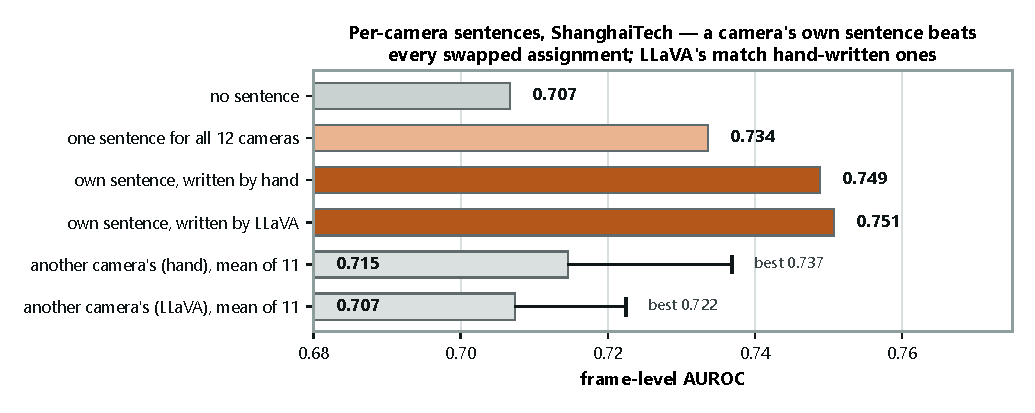
\includegraphics[width=\linewidth]{fig_chart_per_camera}
\caption{Table~\ref{tbl:perview} drawn. Shuffled rows show the mean over the
eleven rotations, with a whisker to the best rotation; both per-camera sets
exceed even the best. The axis begins at $0.68$.}\label{fig:chartperview}
\end{figure}

Both per-view sets beat every one of the eleven shuffled assignments, by
$+0.034$ (hand-written) and $+0.043$ (generated) on average. The benefit
therefore depends on each sentence matching its own camera, which is the scene
identification account of Section~\ref{sec:res-avenue} confirmed by
intervention rather than by partitioning. The gain over the shared sentence,
$+0.015$ and $+0.017$, lies inside the split-to-split spread of
Section~\ref{sec:res-components}, and we report its direction without claiming
its magnitude; the same holds for the difference between the two per-view sets,
which is not evidence that the model writes better descriptions than a person.

What the generated set does establish is that the manual step is not required:
captions produced with no human and no labels match the hand-written set. An
earlier run chose the frames to caption using the ground-truth labels, to avoid
anomalous frames; it gave $0.755$, and removing that dependence changed the
figure by $0.004$. Its captions were visibly imperfect---six of twelve described
people despite the instruction, and two views received identical sentences---so
the method does not appear to need careful descriptions. Deploying to a new camera can therefore consist of
captioning a few frames of its ordinary footage, with no training, no labels and
no human-written text.

\subsection{UCF-Crime under pre-registered predictions}
\label{sec:res-ucf}
ShanghaiTech and Avenue are both campus walkways, and the scene-identification
account was developed on them. UCF-Crime \citep{sultani2018ucfcrime} tests it on
data it was not developed on: its 290 test videos---140 containing one of
thirteen crime classes, 150 normal---come from roughly as many different cameras
and settings, from shop interiors to highways. The protocol and four predictions
were committed to the repository before any UCF-Crime score was computed, and are
reported here as registered.

The configuration is the one used throughout, with three choices fixed in
advance. Every sixteenth frame is scored ($69{,}634$ frames), and the window is
$w{=}5$, the time-equivalent of $w{=}31$ at ShanghaiTech's sampling. The
\texttt{surveillance} prompt ensemble is used unchanged. The primary metric is
frame-level AUROC over raw pooled scores, the convention on this benchmark, with
per-video normalised figures secondary: half the test videos contain no anomaly,
and min--max normalising a video with no anomaly forces some of its frames to the
maximum score. Each video's descriptor is generated by M4 from the video's first
three sampled frames, chosen by position; in 3 of the 140 anomalous videos the
event has begun within them, and those captions are kept, since removing them
would require the labels.

\begin{table}[width=\linewidth,cols=3,pos=htbp]
\caption{UCF-Crime test split, 290 videos, frame-level AUROC. Primary: raw pooled
scores, $w{=}5$. Shuffled rows give each video another video's generated
description, over 20 random derangements.}\label{tbl:ucf}
\begin{tabularx}{\linewidth}{@{}Z l l@{}}
\toprule
\textbf{Descriptor} & \textbf{Raw (primary)} & \textbf{Per-video normalised} \\
\midrule
None & 0.756 & 0.759 \\
Generic & 0.729 & 0.740 \\
One sentence shared by all videos & 0.813 & 0.767 \\
\textbf{Per video, generated by M4} & \textbf{0.824} & \textbf{0.789} \\
Per video, shuffled (mean / best of 20) & 0.713 / 0.779 & 0.741 / 0.784 \\
Mismatched (industrial) & 0.727 & 0.746 \\
\bottomrule
\end{tabularx}
\end{table}

\begin{table}[width=\linewidth,cols=3,pos=htbp]
\caption{The four predictions registered before measurement, and their outcome on
the primary metric.}\label{tbl:ucfpred}
\begin{tabularx}{\linewidth}{@{}Z l l@{}}
\toprule
\textbf{Prediction} & \textbf{Measured} & \textbf{Outcome} \\
\midrule
P1: per-video $-$ mismatched exceeds ShanghaiTech's $+0.105$ & $+0.096$ & \textbf{refuted} \\
P2: per-video beats the shuffled mean & $+0.110$ & holds \\
P3: per-video beats the shared sentence & $+0.011$ & holds (direction) \\
P4: shared beats mismatched & $+0.086$ & holds \\
\bottomrule
\end{tabularx}
\end{table}

\begin{figure}[pos=htbp]
\centering
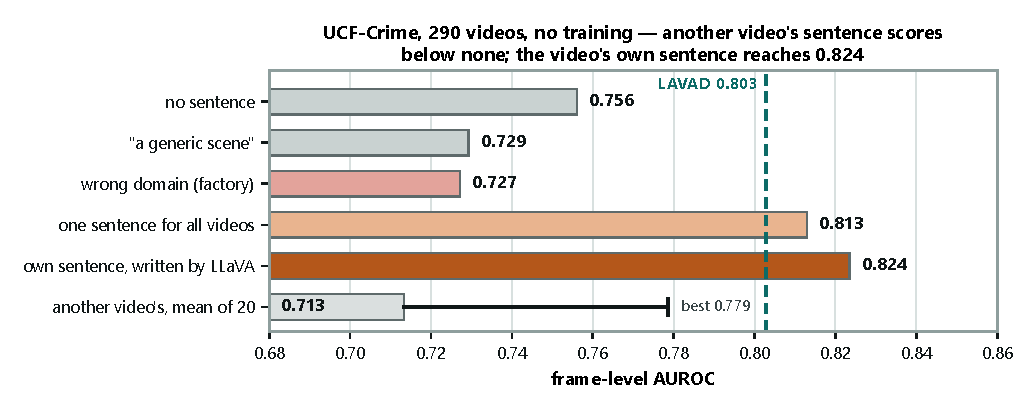
\includegraphics[width=\linewidth]{fig_chart_ucf_crime}
\caption{Table~\ref{tbl:ucf} drawn, primary metric. The shuffled row is the mean
over 20 derangements, with a whisker to the best. The dashed line marks LAVAD's
reported $80.28$ \citep{zanella2024lavad}, which likewise samples every
sixteenth frame; it is a published figure from a different pipeline, not a run
of ours. The axis begins at $0.68$.}\label{fig:chartucf}
\end{figure}

The mechanism transfers, and more strongly than on ShanghaiTech. A video's own
description beats descriptions taken from other videos by $0.110$, against
$0.043$ for ShanghaiTech's cameras, and the shuffled descriptions score below
supplying none at all ($0.713$ against $0.756$): on a benchmark whose scenes
differ this much, the description of another scene is not neutral but
misleading. That is what the scene-identification account predicts, and it is
the strongest single piece of evidence for it in this work.

The quantitative form of the account does not survive. P1 held that the context
gap grows with the scene variety the descriptor must resolve, and so should
exceed ShanghaiTech's $+0.105$ on a benchmark of several hundred scenes. It is
$+0.096$. The within-view reduction of Section~\ref{sec:res-avenue} still stands
---one scene yields a smaller gap than many---but the gap does not keep growing
beyond a dozen scenes, and the claim that the benefit scales with scene diversity
is withdrawn in favour of the weaker one that the benefit requires it.

Two further observations. A single shared sentence already gives most of the
gain here ($0.813$), more than on ShanghaiTech, plausibly because "surveillance
footage of streets, shops and buildings" describes this benchmark's scenes better
than one campus sentence describes twelve walkways. And the per-video normalised
figures are lower throughout, as the registered rationale for the primary metric
anticipated.

The choice of metric matters more than that, and is stated rather than left in
the table. Under per-video normalisation the shared-sentence gap over the
mismatched descriptor shrinks from $+0.086$ to $+0.021$
(Table~\ref{tbl:avenue}), and the per-video descriptors beat the shuffled mean by
$+0.048$ but the best of the twenty derangements by only $+0.005$. The
predictions were registered on the raw metric for the reason given above, and
are reported on it; but on the secondary metric the context effect on UCF-Crime
is markedly weaker, and the claim that it is robust to the evaluation protocol
is not made.

\emph{How certain these figures are.} The 290 test videos were resampled with
replacement 1{,}000 times (seed fixed in the audit script) and every
configuration was scored on the same resamples, so that gaps are measured on
identical data (Table~\ref{tbl:ucfboot}). Resampling videos rather than frames
matters: frames within a video are strongly correlated, and a frame-level
bootstrap would give intervals far narrower than the evidence supports. Only the
comparison with other videos' descriptions has an interval clear of zero. The
gain over no descriptor is positive in $96.6\%$ of resamples but its interval
touches zero, and the gain over the shared sentence is not distinguishable from
zero, as already reported.

\begin{table}[width=\linewidth,cols=4,pos=htbp]
\caption{UCF-Crime, paired video-level bootstrap (1{,}000 resamples of the 290
test videos). Raw pooled AUROC, $w{=}5$. LAVAD and AnyAnomaly are fixed
published figures; their own uncertainty is not available, so only this work's
side is resampled.}
\label{tbl:ucfboot}
\begin{tabularx}{\linewidth}{@{}Z l l l@{}}
\toprule
\textbf{Quantity} & \textbf{Estimate} & \textbf{95\% interval} & \textbf{Resamples $>0$} \\
\midrule
Per-video descriptors, AUROC & $0.824$ & $[0.756, 0.877]$ & --- \\
Per-video $-$ none & $+0.067$ & $[-0.002, +0.153]$ & $96.6\%$ \\
Per-video $-$ shared sentence & $+0.011$ & $[-0.047, +0.080]$ & $55.3\%$ \\
Per-video $-$ other videos' (mean of 20) & $+0.110$ & $[+0.069, +0.157]$ & $100\%$ \\
\midrule
AUROC above LAVAD's $0.803$ & \multicolumn{3}{l}{in $72.8\%$ of resamples} \\
AUROC above AnyAnomaly's $0.807$ & \multicolumn{3}{l}{in $67.3\%$ of resamples} \\
\bottomrule
\end{tabularx}
\end{table}

\emph{Relation to LAVAD.} LAVAD \citep{zanella2024lavad}, the closest
training-free pipeline, reports $80.28$ AUROC on this benchmark, and AnyAnomaly
reports $80.7$ \citep{anyanomaly2025}. The per-video figure of $82.4$ is
numerically above both, but the bootstrap places it above them in only about
seven resamples in ten (Table~\ref{tbl:ucfboot}): the difference is inside this
work's own uncertainty, before any cross-paper protocol difference is
considered. The sampling matches: LAVAD also samples each
video every sixteen frames. Two differences remain. LAVAD does not state whether
its frame-level AUROC is computed over the sampled frames, as here, or with
scores propagated to every frame; and its pipeline chains a captioner, a large
language model and a cross-modal refinement stage, where this one uses a single
frozen encoder pass per sampled frame and one caption per video. A margin of two
points across papers is within what such protocol details can move, and within
the bootstrap interval, so we report the comparison as comparable, not as a win.

\subsection{What the descriptor changes: a measurement audit}
\label{sec:res-audit}
Every context gap above is a difference in pooled AUROC, which ranks the frames
of all videos against one another. A descriptor can raise that figure in two
different ways: by \emph{re-ranking} frames inside a video, so that its
anomalous frames move above its normal ones, or by \emph{calibration}---moving
each video's scores up or down as a block, so that frames from different cameras
become comparable while the order inside every video stays the same. Two earlier
observations pointed to calibration: on ShanghaiTech at $w{=}5$ the
matched--mismatched gap is $+0.100$ pooled but $+0.006$ when AUROC is computed
within each video, and scoring the raw cosine margin instead of the softmax cuts
the pooled gap at $w{=}31$ to $+0.017$.

The audit measures the question directly. For each pair of conditions it splits
the pooled gap exactly into a \emph{level} part---what the reference condition
gains when each of its videos is shifted by the mean change in that video's
margin, its within-video pattern kept---and the remainder, averaged over both
orders so that the split does not depend on which condition comes first. Within-
video ranking is measured on the smoothed margin, which a per-video shift cannot
change. The decision rule was committed with the script before any audit number
existed: a gap is \emph{calibration-dominated} if its level share is at least
$2/3$ and the within-video change is at most a third of the gap, and
\emph{re-ranking-dominated} if the level share is at most $1/3$. Before
reporting anything, the script reproduced the published figures of every
condition on the benchmarks it covers (52 checks, all passed).

\begin{table}[width=\linewidth,cols=6,pos=htbp]
\caption{Measurement audit. Level: the part of the pooled gap reproduced by a
per-video score shift alone. Within: change in mean within-video AUROC of the
smoothed margin. ShanghaiTech per-clip normalised, $w{=}31$; UCF-Crime raw,
$w{=}5$. Shuffled rows average 11 (ShanghaiTech) and 20 (UCF-Crime) controls.}
\label{tbl:audit}
\begin{tabularx}{\linewidth}{@{}Z l l l l l@{}}
\toprule
\textbf{Comparison} & \textbf{Gap} & \textbf{Level} & \textbf{Share} & \textbf{Within} & \textbf{Verdict} \\
\midrule
ShanghaiTech, matched $-$ mismatched & $+0.105$ & $+0.086$ & $0.82$ & $+0.006$ & calibration \\
ShanghaiTech, per-camera $-$ shuffled & $+0.043$ & $+0.015$ & $0.34$ & $+0.010$ & mixed \\
UCF-Crime, per-video $-$ none & $+0.067$ & $+0.056$ & $0.83$ & $+0.001$ & calibration \\
UCF-Crime, per-video $-$ shuffled & $+0.110$ & $+0.096$ & $0.87$ & $+0.024$ & calibration \\
\bottomrule
\end{tabularx}
\end{table}

Table~\ref{tbl:audit} gives the result. The three headline gaps are
calibration-dominated: $82$--$87\%$ of each is a per-video level shift, and the
within-video ranking moves by at most $+0.024$. On ShanghaiTech, CLIP's logit
scale amplifies that shift: recomputed with the softmax temperature at
$\lambda{=}1$, $10$, $30$, $100$ and $300$, the matched--mismatched gap is
$+0.017$, $+0.022$, $+0.047$, $+0.105$ and $+0.133$. On UCF-Crime, scored raw,
it barely depends on $\lambda$ ($+0.057$ at $\lambda{=}1$, $+0.067$ at $100$):
there the calibration acts directly on the pooled ranking rather than through
the softmax.

Per-camera descriptors on ShanghaiTech are the exception. Only a third of their
advantage over swapped descriptors is a level shift; the remainder survives
removing each video's level and scale (the per-clip-normalised raw margin keeps
$+0.025$), although within-video ranking improves by only $+0.010$. A camera's
own sentence therefore changes the shape of its videos' scores, not merely their
level, without much reordering of frames inside a video.

Calibration is not something a trivial rule recovers. Subtracting each video's
own mean margin before scoring---a label-free, sentence-free per-video
calibration---gives $0.657$ on ShanghaiTech and $0.702$ on UCF-Crime, below no
descriptor at all ($0.707$, $0.756$) and well below the per-camera and
per-video descriptors ($0.751$, $0.824$). The descriptor places each camera on a
common scale in a way that removing its offset does not.

This changes what the earlier results mean, not what they measured. The
descriptor does not chiefly redefine what is normal inside a scene; it tells the
scorer which scene it is looking at, and in doing so puts different cameras on
one scale. That is what a deployment with a single alarm threshold across many
cameras requires, and it is consistent with every result above: no effect on a
single camera (Avenue), a small effect within one view, gains from per-camera
sentences and harm from swapped ones. It also bears on the metric. A gap of
$+0.105$ under the softmax is $+0.017$ under the margin beneath it, so pooled
AUROC from CLIP softmax scores can report large differences that within-video
ranking does not show---a caution for any CLIP-based detector evaluated this way.

\subsection{Where it fails: XD-Violence and NWPU Campus}
\label{sec:res-xd}
Two further benchmarks test the account at its edges. XD-Violence
\citep{wu2020xdviolence} mixes films, sports, games, news and CCTV, so many of its
videos have no fixed scene at all, and is scored by frame-level average precision,
its official measure. NWPU Campus \citep{cao2023nwpu} has 43 campus scenes and
includes anomalies that are anomalous only in particular scenes---the case concept
shift describes most directly. The pipeline is unchanged (CLIP ViT-L/14, every
sixteenth frame, $w{=}5$, raw scores). Each XD-Violence video receives a description
generated by M4 from its first three sampled frames, as on UCF-Crime; each NWPU scene
receives one from the first video of that scene. The shared descriptions are
``scenes from films, television, news, sports and online videos'' and ``a university
campus with roads, footpaths, squares and buildings''.

\begin{table}[width=\linewidth,cols=3,pos=htbp]
\caption{XD-Violence (800 test videos, average precision) and NWPU Campus (242 test
videos, frame-level AUROC). Differences are paired against no description over
1{,}000 video-level resamples; ``shuffled'' gives each video or scene another one's
generated description (mean over five derangements).}\label{tbl:xdnwpu}
\begin{tabularx}{\linewidth}{@{}Z l l@{}}
\toprule
\textbf{Description} & \textbf{XD-Violence (AP)} & \textbf{NWPU Campus} \\
\midrule
None & 0.624 & 0.659 \\
One shared description & 0.582 & 0.648 \\
Generated per video (XD) or per scene (NWPU) & \textbf{0.417} & 0.667 \\
Generated, shuffled & 0.454 & 0.601 \\
\midrule
Generated $-$ none & $-0.207$ $[-0.261, -0.155]$ & $+0.008$ $[-0.025, +0.043]$ \\
Shared $-$ none & $-0.042$ $[-0.067, -0.020]$ & $-0.011$ $[-0.039, +0.019]$ \\
Generated $-$ shuffled & $-0.036$ $[-0.083, +0.009]$ & $+0.066$ $[+0.014, +0.109]$ \\
\bottomrule
\end{tabularx}
\end{table}

\emph{XD-Violence: the description names the anomaly.} The generated description
lowers average precision from $0.624$ to $0.417$ (Table~\ref{tbl:xdnwpu}), and a
video's own description is no better than another video's. The cause is in the frames
the description is written from. In 127 of the 500 violent test videos the violence
has already begun within the first three sampled frames, so the caption that is meant
to state what is normal in the scene describes the event, and the detector is told
that the anomaly is normal. An exploratory analysis, which uses the labels and is not
a pre-registered test, confirms the mechanism: removing the description from those
127 videos alone recovers $66\%$ of the loss ($0.417 \to 0.554$), whereas removing it
from videos whose captions contain violent words recovers $7\%$. On UCF-Crime the same
situation arose in 3 of 140 anomalous videos (Section~\ref{sec:res-ucf}); here it is a
quarter of them. By the audit of Section~\ref{sec:res-audit}, the loss is again mostly
a shift in score level ($69\%$), now in the wrong direction.

\emph{NWPU Campus: scene identity without a gain.} The per-scene descriptions neither
help nor hurt ($+0.008$, interval spanning zero), although a scene's own description
beats another scene's significantly ($+0.066$). This is the calibration account of
Section~\ref{sec:res-audit} in a sharper form: a wrong scene costs accuracy, as on
ShanghaiTech and UCF-Crime, but on this benchmark the right one adds nothing to the
plain detector. Forty-three scenes are therefore not sufficient for a description to
help, which narrows the scene-diversity account of Section~\ref{sec:res-avenue}
further: diversity is necessary but not sufficient.

\emph{What the failures imply.} A description written from a camera's opening
footage is only as good as that footage. Where the opening frames can contain the
event---footage that starts mid-incident, edited video, a camera installed during an
incident---the description can do more harm than none. Any method that summarises a
scene from its first frames inherits this risk. A remedy has to describe normality
without depending on what the opening frames show.

\subsection{Full ROC and precision--recall curves}
\label{sec:res-roc}
Every figure above is the area under a curve. Figure~\ref{fig:roc} shows the
curves themselves, on the four multi-scene benchmarks, for three description
conditions: no description, one shared description, and the description generated by M4 per
camera (ShanghaiTech), per video (UCF-Crime, XD-Violence) or per scene (NWPU
Campus). The areas reproduce the published figures to within $0.001$.

The curves show where each gain or loss is made. On UCF-Crime the descriptions
raise the true-positive rate most at low and moderate false-positive rates: at a
false-positive rate of $0.2$ it rises from about $0.5$ with no description to
about $0.7$ with the generated one, and the curves meet again beyond $0.5$, so
the gain lies in the operating range a deployment would use. On ShanghaiTech the
generated and shared descriptions lie above the no-description curve over most
of its length, by a smaller margin. On NWPU Campus the curves cross: the shared
description is below the plain detector at low false-positive rates and above it
later, which is why their areas differ by only $0.011$. On XD-Violence the
generated description lowers precision at almost every level of recall, not only
in one region, which is the signature of the uniform score shift diagnosed in
Section~\ref{sec:res-xd}.

\begin{figure}[pos=htbp]
\centering
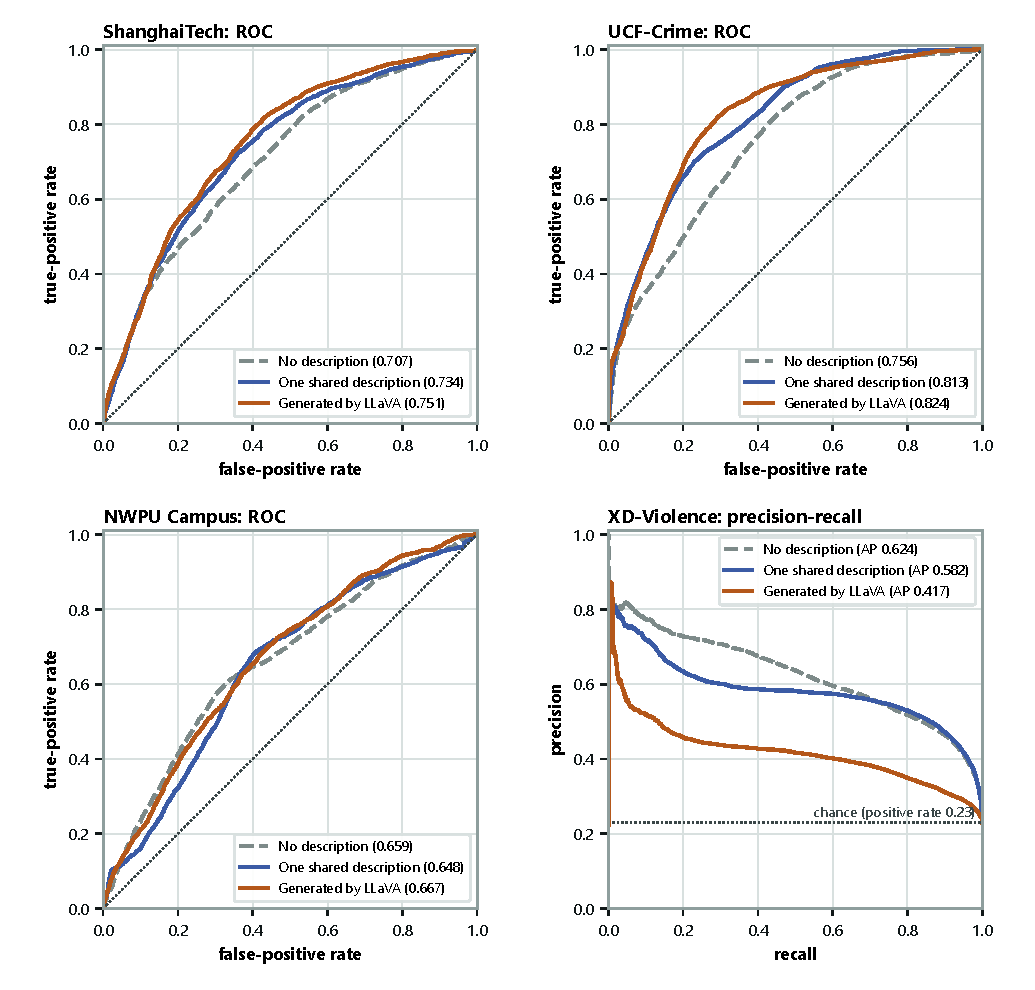
\includegraphics[width=\linewidth,height=0.70\textheight,keepaspectratio]{fig_roc_curves}
\caption{ROC curves (ShanghaiTech, UCF-Crime, NWPU Campus) and the
precision--recall curve (XD-Violence, whose official measure is average
precision) for the frozen CLIP ViT-L/14 pipeline with no description, one shared
description, and the description generated by LLaVA. ShanghaiTech: $w{=}31$,
per-clip normalised; the others: $w{=}5$, raw pooled. Areas in the legends are
those reported in Tables~\ref{tbl:perview}, \ref{tbl:ucf} and~\ref{tbl:xdnwpu}.
Dotted lines mark chance: the diagonal for ROC, and the proportion of anomalous
frames ($0.23$) for precision--recall.}\label{fig:roc}
\end{figure}

\subsection{Comparison with published methods on the same benchmarks}
\label{sec:res-comparison}
All five video benchmarks used here are standard, so published figures are
available for comparison. Table~\ref{tbl:sota} groups methods by \emph{what each
requires of the target scene}, because that is the axis along which they are not
interchangeable: a detector that has trained on normal video from ShanghaiTech
and one that has seen nothing of it are not solving the same problem, and a
single ranking would misrepresent both. Figure~\ref{fig:comparison} draws the
same numbers, one panel per benchmark.

Every external figure was read from a source paper, and where possible from one
that tabulates several methods under a single protocol. The CUHK Avenue and
ShanghaiTech figures, and the UCF-Crime figures for FPDM, MULDE and AnyAnomaly,
are from Tables~5 and~6 of \citet{anyanomaly2025}; LAVAD and its zero-shot
baselines on UCF-Crime and XD-Violence are from Tables~1 and~2 of
\citet{zanella2024lavad}; the NWPU Campus figures are from Table~4 of
\citet{cao2023nwpu}; and the more recent training-free methods are from their
own papers. Cross-paper comparisons carry protocol differences that a table
cannot remove, and the text below names them where they matter.

\begin{table}[width=\linewidth,cols=6,pos=htbp]
\caption{Published results on the five video benchmarks, grouped by what the
method requires of the target scene: frame-level AUROC (\%), except XD-Violence,
where it is average precision (\%), that benchmark's official measure. A dash
means the benchmark is not reported. Sources: CUHK Avenue and ShanghaiTech, and
UCF-Crime for FPDM, MULDE and AnyAnomaly, as tabulated by
\citet{anyanomaly2025}; $^{\dagger}$the benchmark's own baseline, from the paper
introducing it; $^{\ddagger}$as tabulated by \citet{zanella2024lavad}, whose
zero-shot baselines are built independently of those of \citet{anyanomaly2025}
(ImageBind is its image-encoder variant); $^{\P}$as tabulated by
\citet{cao2023nwpu}, computed over every frame, where ours uses every sixteenth;
the remaining rows from each method's own paper (the frozen-VLM row is the mean
over four VLMs scored by the probability of answering ``yes''). Ours, no
description: the frozen pipeline alone. $^{\S}$Ours, with description: the
configuration the method proposes, one shared sentence on CUHK Avenue and
ShanghaiTech (Table~\ref{tbl:avenue}), the description generated per video on
UCF-Crime and XD-Violence and per scene on NWPU Campus. Bold: best training-free
entry per benchmark.}\label{tbl:sota}
\small
\begin{tabularx}{\linewidth}{@{}Z c c c c c@{}}
\toprule
\textbf{Method} & \textbf{CUHK Avenue} & \textbf{ShanghaiTech} & \textbf{UCF-Crime} &
\textbf{XD-Violence} & \textbf{NWPU Campus} \\
\midrule
\multicolumn{6}{@{}l}{\emph{One-class --- normal video from the target scene, plus a training run}} \\
Liu et al. \citep{liu2018shanghaitech}$^{\dagger}$ & 85.1 & 72.8 & --- & --- & --- \\
MPN \citep{lv2021mpn} & 89.5 & 73.8 & --- & --- & 64.4$^{\P}$ \\
FPDM \citep{yan2023fpdm} & 90.1 & 78.6 & 74.7 & --- & --- \\
MA-PDM \citep{zhou2024mapdm} & 91.3 & 79.2 & --- & --- & --- \\
MULDE \citep{micorek2024mulde} & --- & 81.3 & 78.5 & --- & --- \\
Cao et al., scene-conditioned \citep{cao2023nwpu} & --- & --- & --- & --- & 68.2$^{\P}$ \\
\midrule
\multicolumn{6}{@{}l}{\emph{Few-shot --- a few normal frames from the target scene, and GPT-4}} \\
AnomalyRuler \citep{yang2024anomalyruler} & --- & 85.2 & --- & --- & --- \\
\midrule
\multicolumn{6}{@{}l}{\emph{Training-free --- no target data, no gradient updates}} \\
Zero-shot CLIP \citep{radford2021clip} & 62.3 & 60.9 & 53.2$^{\ddagger}$ & 17.8$^{\ddagger}$ & --- \\
Zero-shot ImageBind \citep{girdhar2023imagebind} & 64.5 & 61.3 & 53.7$^{\ddagger}$ & 27.3$^{\ddagger}$ & --- \\
LLaVA-1.5 \citep{liu2023llava} & 67.4 & 59.6 & 72.8$^{\ddagger}$ & 50.3$^{\ddagger}$ & --- \\
Video-ChatGPT \citep{maaz2024videochatgpt} & 76.9 & 69.1 & --- & --- & --- \\
LAVAD \citep{zanella2024lavad} & --- & --- & 80.3$^{\ddagger}$ & 62.0$^{\ddagger}$ & --- \\
AnyAnomaly \citep{anyanomaly2025} & \textbf{87.3} & \textbf{79.7} & 80.7 & --- & --- \\
Frozen VLM, yes/no score \citep{song2026vlmanswer} & --- & --- & 85.3 & 69.0 & --- \\
Flashback-PE \citep{lee2025flashback} & --- & --- & 87.3 & 75.1 & --- \\
ASK-Hint \citep{zou2026askhint} & --- & --- & 89.8 & --- & --- \\
NOVA \citep{yin2026nova} & --- & --- & \textbf{89.9} & \textbf{84.8} & --- \\
DA-ZVAD, no description (ours) & 70.6 & 70.7 & 75.6 & 62.4 & 65.9 \\
DA-ZVAD, with description (ours)$^{\S}$ & 67.7 & 73.4 & 82.4 & 41.7 & \textbf{66.7} \\
\bottomrule
\end{tabularx}
\end{table}

\begin{figure}[pos=htbp]
\centering
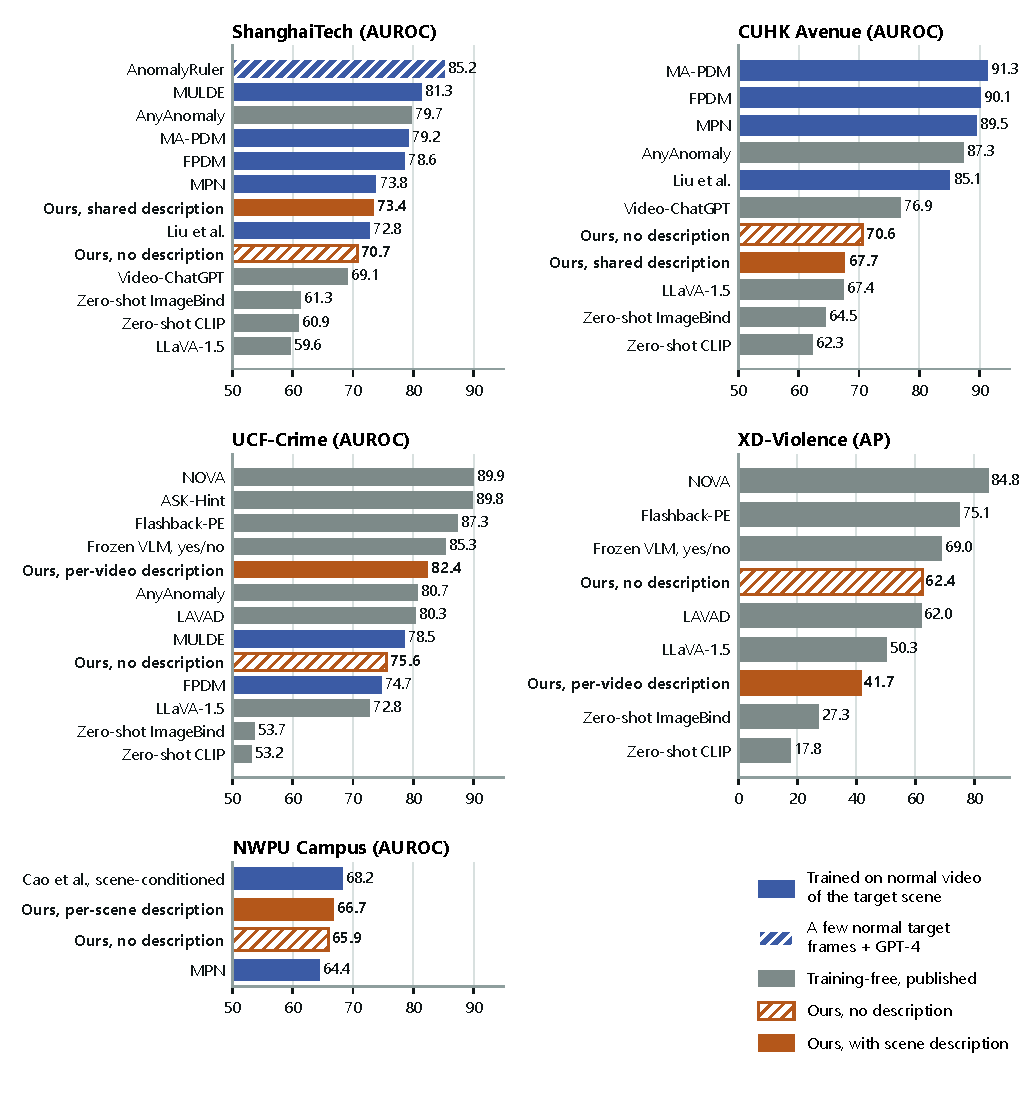
\includegraphics[width=\linewidth,height=0.72\textheight,keepaspectratio]{fig_comparison}
\caption{Table~\ref{tbl:sota} drawn, one panel per benchmark, each sorted by
score. Blue: methods that use normal video or frames of the target scene; grey:
published training-free methods; orange: this work, hatched without a
description and solid with the proposed description. The AUROC axes begin at 50,
which is chance; XD-Violence is scored by average precision, whose chance level
is the proportion of anomalous frames. Cross-paper protocol caveats are given in
the caption of Table~\ref{tbl:sota}.}\label{fig:comparison}
\end{figure}

\subsubsection{Where the present work sits}
Against the other training-free entries, the position depends on the benchmark.
On ShanghaiTech this work is second of six, behind AnyAnomaly, and on CUHK
Avenue third of six. On UCF-Crime it is fifth of ten: above LAVAD and AnyAnomaly
by a margin inside its own bootstrap interval, so comparable to them rather than
ahead (Table~\ref{tbl:ucfboot}), and below four more recent methods---frozen-VLM
yes/no scoring ($85.3$), Flashback ($87.3$), ASK-Hint ($89.8$) and NOVA
($89.9$). Those methods invest in the text and the reasoning side: prompt banks
written per anomaly class, action-centric prompts, memories of generated
captions, or a large VLM queried per frame. None of them tests what a
description of the deployment scene contributes, which is the question this
paper asks, and their gains are not in tension with its findings. On UCF-Crime
the figure also exceeds the two one-class methods that report it (FPDM $74.7$,
MULDE $78.5$), both of which train on that benchmark's normal footage.

On XD-Violence the frozen pipeline alone reaches $62.4$ AP, level with LAVAD's
$62.0$ and below the more recent methods ($69.0$--$84.8$); the generated
description lowers it to $41.7$, the failure analysed in
Section~\ref{sec:res-xd}, and the only benchmark on which the proposed
configuration ranks below the plain LLaVA-1.5 baseline. On NWPU Campus no
training-free method in Table~\ref{tbl:sota} reports a figure. There our $66.7$
lies inside the band of one-class methods that train on the benchmark's normal
footage, above MPN ($64.4$) and below the scene-conditioned model of
\citet{cao2023nwpu} ($68.2$); their figures are computed over every frame and
ours over every sixteenth, so the comparison is indicative only.

The one-class rows are included because they set the scale, and because the
cost they pay is the quantity this work is trying to remove. Each of them
consumes hours of normal video from the target scene plus a training run before
it produces its first score; AnomalyRuler needs only a few normal frames, but
also a GPT-4 reasoning stage.

Read against that band, $73.4$ on ShanghaiTech exceeds the benchmark's own
baseline \citep{liu2018shanghaitech}, which reaches $72.8$ \emph{by training on
ShanghaiTech's training split}, and sits alongside MPN ($73.8$). It falls below
the later diffusion- and density-based methods, which reach $78$--$81$. So the
claim is bounded and specific: training-free scoring with a supplied scene
description reaches the level of the benchmark's established baseline at no
target-data cost, and does not approach the current one-class state of the art.
On CUHK Avenue it does not reach that band at all ($67.7$ against $85.1$), which
is the single-scene limitation of Section~\ref{sec:res-avenue} appearing again.

\subsubsection{Why the Avenue figure trails the field while ShanghaiTech does not}
\label{sec:res-whyavenue}
Table~\ref{tbl:sota} shows an asymmetry worth accounting for: on ShanghaiTech
this work sits second among the training-free entries and above the benchmark's
own trained baseline, whereas on Avenue it sits third and well below the
one-class band. Two separate effects produce that, and only one of them is the
scene-diversity limitation already reported.

\emph{The detector itself does not degrade.} With no descriptor the two
benchmarks give $0.706$ and $0.707$ (Table~\ref{tbl:avenue}). Whatever is
happening on Avenue is not a failure of the frozen encoder to transfer; the
base detector performs identically on both.

\emph{Effect one: the descriptor has nothing to resolve.} Avenue is a single
fixed view, so a scene description cannot perform the discrimination it performs
across ShanghaiTech's twelve views. The matched condition therefore falls
\emph{below} the ungrounded one ($0.677$ against $0.706$), and the within-view
control of Section~\ref{sec:res-avenue} shows the same collapse inside a single
ShanghaiTech view. This accounts for the loss relative to our own ShanghaiTech
figure but not for the distance to the other methods.

\emph{Effect two, and the larger one: Avenue's anomalies are of a kind
whole-frame semantic matching cannot express.} The two benchmarks differ in what
their anomaly classes \emph{are}, not merely in how many scenes they span.
ShanghaiTech's appearance classes are object categories a web-scale
image--text model represents directly---car, bicycle, motorcycle, hand
truck---and asking whether a frame contains a bicycle is close to the task CLIP
was trained on. Avenue's appearance classes are bicycle and ``too close'',
the latter being a property of the object's distance from the camera rather
than of its identity; no phrasing of a scene description expresses it, because
the frame contains nothing that is semantically out of place. Its remaining
classes---throwing, running, dancing---are brief, small in the frame, and
defined by motion rather than by content.

This is the resolution limitation identified on MVTec~AD
(Section~\ref{sec:res-mvtec}) reappearing on video: pooled whole-frame embeddings
at $224\times224$ capture what a scene contains and not how large, how fast, or
how near it is. It also explains why the one-class band is \emph{higher} on
Avenue ($85$--$91$) than on ShanghaiTech ($73$--$81$) while ours is lower: a
model trained on Avenue's own normal footage learns that scene's characteristic
scale and motion statistics, which is precisely the information a frozen
semantic encoder discards.

The reading we take from this is that the method is suited to anomalies that are
semantic---something present that does not belong---and unsuited to anomalies
that are geometric or kinematic, and that this distinction predicts benchmark
performance better than benchmark difficulty does. Patch-level scoring against
the encoder's spatial tokens, listed in Section~\ref{sec:conclusion}, addresses
the first half of that gap; the second half is a limitation of the
representation rather than of the scoring rule.

\subsubsection{Why the plain vision-language baselines score lower, and what
that does \emph{not} establish}
The four plain vision-language baselines in Table~\ref{tbl:sota} (zero-shot CLIP, zero-shot ImageBind, LLaVA-1.5 and Video-ChatGPT) are instructive, and the reason they score lower is largely not the scene
descriptor. It is worth stating precisely, because the natural reading of the
table overstates the case.

The zero-shot CLIP baseline is a close relative of this pipeline's M1 stage with
everything else stripped away. \citet{zanella2024lavad}, who construct the same
baseline, describe it as scoring each frame by the softmax over its cosine
similarity to two single prompts---``a standard scene'' and ``a scene with
suspicious or potentially criminal activities''---on a ViT-B/32 backbone. This
pipeline differs from that in four respects before any domain descriptor is
involved: it ensembles several phrasings per side rather than using one prompt
\citep{jeong2023winclip}; it smooths over a $31$-frame window
(Section~\ref{sec:res-video}, worth roughly four points); it normalises each clip
before pooling, which Table~\ref{tbl:video} shows is worth close to twenty
points on this benchmark; and it uses the larger ViT-L/14.

The decomposition matters. With \emph{no} descriptor at all this pipeline scores
$0.707$ (Table~\ref{tbl:sweep}), already $9.8$ points above zero-shot CLIP. The
descriptor moves it from $0.707$ to $0.734$, a further $2.7$ points, and
Section~\ref{sec:res-sweep} reports that this margin sits inside the
split-to-split spread and declines to claim its magnitude. \textbf{The gap
between this work and the plain zero-shot baselines is therefore mostly
attributable to protocol and scale, not to verbalised context.} The evidence
that the descriptor is load-bearing remains the mismatched condition---a wrong
description costs $0.105$---and not the margin over external baselines.

LLaVA-1.5 and Video-ChatGPT are substantially larger models scoring below or
near this pipeline, which is a comment on task fit rather than on capacity: both
are general-purpose conversational models asked to emit a score, and neither is
constructed to produce a well-ordered ranking over frames, which is what AUROC
measures.

\subsubsection{Against AnyAnomaly}
AnyAnomaly \citep{anyanomaly2025} is the closest published work and leads the training-free entries on both campus benchmarks. Three differences the AUROC column does not show are worth
recording.

\emph{The supplied text points the opposite way.} AnyAnomaly implements
\emph{customizable} VAD: the operator names what is \emph{abnormal}---
``bicycle'', ``fighting'', ``jumping-falling''---and each frame is scored for the
presence of that event. This work supplies a description of what is
\emph{normal} in the deployment scene, and an anomaly is a departure from it.
The distinction matters because \citet{anyanomaly2025} open by noting that
abnormal events are ``rare and diverse, making it difficult to construct
large-scale datasets''; a method requiring the operator to enumerate them in
advance inherits that difficulty, whereas a description of normality does not.

\emph{The benchmark evaluation supplies the anomaly taxonomy.} To obtain the
figures in Table~\ref{tbl:sota}, \citet{anyanomaly2025} state that ``each
anomaly class in the dataset was treated as $X$, and the maximum anomaly score
among all computed scores was assigned to the corresponding segment.'' The
method is told, per benchmark, which anomaly classes to look for and scored on
the maximum over them. The present method receives a description of the scene
and no information about the anomaly classes. The two rows do not describe
equally informed systems.

\emph{The inference budget differs by roughly an order of magnitude.}
AnyAnomaly issues three large vision-language model queries per
segment---representative key frame, position context and temporal
context---having first run CLIP for key-frame selection and multi-scale
windowing to construct them. This pipeline runs one frozen CLIP pass per frame
and reads one sentence, within roughly $7$\,GB.

\subsubsection{What this work solves that the comparison set does not}
\label{sec:res-openset}
Table~\ref{tbl:sota} invites the reading that this work is a weaker AnyAnomaly.
It is not: the two answer different questions, and the difference is the one that
motivates anomaly detection in the first place.

\emph{The two methods require opposite things of the operator.} AnyAnomaly
implements \emph{customizable} VAD, in which the operator names the event to be
detected---``bicycle'', ``fighting'', ``jumping-falling''---and each frame is
scored for the presence of that event. Detection is therefore closed over the
supplied vocabulary: an event the operator did not anticipate produces no
score, because nothing in the pipeline is looking for it. This work supplies a
description of what is \emph{normal} in the deployment scene and flags departure
from it, which is the one-class formulation carried into a zero-shot setting.
Its detection surface is not enumerated in advance.

The asymmetry is stark when stated as a deployment requirement.
\begin{itemize}
  \item AnyAnomaly asks: \emph{list the things that could go wrong here.}
  \item This work asks: \emph{describe what ordinarily happens here.}
\end{itemize}
An operator can always do the second. The first is precisely what
\citet{anyanomaly2025} identify as intractable in their own opening---abnormal
events are ``rare and diverse, making it difficult to construct large-scale
datasets''---and enumerating them in a prompt inherits that difficulty rather
than removing it.

\emph{This bears directly on how Table~\ref{tbl:sota} should be read.} The
figures reported for AnyAnomaly are obtained by treating ``each anomaly class in
the dataset'' as the query and taking the maximum score across them. The
benchmark's anomaly taxonomy is therefore supplied to the method at evaluation
time. That is a reasonable protocol for the task it defines, and it is the task
its authors set out to solve. It does mean that $79.7$ measures closed-set
performance with the class list provided, and is not evidence about behaviour at
a deployment where the class list is unknown---which is the setting the present
work targets. No claim is made here that this pipeline would exceed AnyAnomaly
under a withheld taxonomy; that experiment has not been run, and it is named in
Section~\ref{sec:conclusion} as the most informative one available.

\subsubsection{Two findings that transfer beyond this pipeline}
Framing the contribution as ``a control the others did not run'' understates it,
because the control produced results that apply to any text-conditioned
detector, including the methods in Table~\ref{tbl:sota}.

\emph{Where the text enters dominates what the text says.} Injecting the same
descriptor into both prompt ensembles rather than the normal ensemble alone
moves the matched-minus-mismatched contrast from $-0.029$ to $+0.105$: the
effect changes sign. The mechanism, prototype dilution under mean pooling
(Section~\ref{sec:res-sweep}), is a property of ensemble-and-pool prompt
construction generally, not of this implementation. Any study reporting that
scene descriptions fail to help, without varying the fusion rule, has reported
an artefact of an implementation detail. This work nearly did, and the record of
that inversion is in Table~\ref{tbl:sweep}.

\emph{Verbalised context needs scene diversity to resolve.} The context gap is
$+0.105$ pooled across twelve ShanghaiTech views, $+0.033$ within a single view,
and $+0.020$ on single-view Avenue (Table~\ref{tbl:withinview}). That is a
prescriptive statement about where such methods should be deployed---installations
spanning several environments, not fixed single-camera sites---and it was obtained
by measurement rather than by argument from benchmark identity. A stronger,
proportional form of it was registered and tested on UCF-Crime and did not hold
(Section~\ref{sec:res-ucf}): several hundred scenes gave a gap no larger than
twelve.

Neither finding is available without a condition in which the supplied text is
deliberately wrong while everything else is held fixed. That condition is the
instrument; these two results are what it produced.

% =====================================================================
\section{Discussion and Conclusion}
\label{sec:conclusion}
% =====================================================================

The analytical position of this work rests on four points, each established in
Sections~\ref{sec:lit}--\ref{sec:contrib} and unaffected by the experiments that
follow them.

\begin{itemize}
  \item The domain-adaptation literature targets covariate shift by explicit
        scoping decision, and its theoretical conditions assume the conditional
        $p(y\mid x)$ to be stable.
  \item Anomaly detection violates that assumption structurally, because
        normality is defined by deployment context; concept shift is therefore
        its dominant form of domain shift.
  \item Vision-language foundation models absorb much of the covariate shift that
        motivated the classical toolkit, relocating the operative difficulty to
        the shift type the literature set aside.
  \item A fully frozen pipeline makes the adaptation claim identifiable: with no
        parameters updated, an effect can be attributed to the supplied text.
\end{itemize}

Eight empirical findings follow from the experiments completed to date.

\emph{Verbalised context is load-bearing, and the evidence is the falsifying
control rather than the positive one.} Supplying a descriptor of the wrong
domain costs $0.105$ AUROC, while supplying the correct one improves on
supplying none by $0.027$---a margin that is positive at every temporal window
and grows with it, but which lies inside the split-to-split spread and is
therefore reported as a direction rather than a magnitude. The asymmetry matters
for how the mechanism should be understood: the descriptor is not adding
information that lifts detection so much as constraining a decision boundary
that degrades measurably when misdirected. Since no parameter is free to vary,
the deficit is attributable to the text alone.

\emph{The point of injection dominates the wording.} Appending the descriptor to
both prompt ensembles rather than to the normal ensemble alone reverses the
direction of the effect, because mean-pooled ensembles sharing a common textual
component yield prototypes drawn toward one another. The same mechanism accounts
for a domain-specific prompt ensemble underperforming a minimal pair of prompts
sharing no vocabulary. Verbalised adaptation is consequently more fragile than
its framing in the literature suggests: a study reporting that scene
descriptions do not help, without varying the fusion rule, would have reported
an artefact of an implementation detail.

\emph{The minimal configuration is the best one, and this was established by
failing to improve on it.} Six modifications were tested against the plain
frozen-encoder pathway---scene-conditioned normality, kinematic scoring, local
temporal deviation, quadrant-level scoring, per-prompt maximum pooling, and a
domain-specific prompt ensemble---and none improved on it. Two of them raised a
component score in isolation while reducing the measured contribution of the
descriptor, which is the more interesting failure: on this evidence the
modifications that make the detector better make the text matter less. A single
frozen encoder, two prompt ensembles, a moving average and one sentence is not a
simplification of the method for presentation; it is what survived the
alternatives.

\emph{The adaptation mechanism is bounded, and we can say what bounds it.}
Applied unchanged to CUHK Avenue, the framework detects equally well ($0.706$
against $0.707$) but its context effect nearly vanishes: the gap falls from
$+0.105$ to $+0.020$ and an accurate descriptor scores below no descriptor at
all. Avenue is a single camera view where ShanghaiTech is twelve. Confining
the ShanghaiTech evaluation to one view at a time reproduces the flat result
($+0.033$ against $+0.105$ pooled), which supports the reading directly rather
than by analogy between benchmarks. What the descriptor mainly supplies is the
identification of which environment is in view, not a characterisation of
normality within it. This scopes the claim rather than abandoning it, and it
predicts where verbalised adaptation should and should not be expected to
help---in deployments spanning several environments, and not in a fixed
single-camera installation.

\emph{The descriptor can be written by the system itself.} A sentence per camera,
generated by the frozen multimodal model from a few ordinary frames, reaches
$0.751$ against $0.734$ for one sentence shared by every camera, and the gain
disappears when the sentences are exchanged between cameras. The gain over the
shared sentence is within the noise and is reported as a direction; what is
established is that the benefit depends on each sentence matching its camera,
and that producing those sentences needs no human.

\emph{The mechanism holds on data it was not developed on; its quantitative
form does not.} On UCF-Crime, under predictions registered in advance, a
video's own generated description beats descriptions taken from other videos by
$0.110$ and reaches $0.824$, while descriptions of other scenes score below none.
The prediction that the effect would grow with scene diversity beyond
ShanghaiTech's was refuted: the gap is $+0.096$ against $+0.105$. The claim is
accordingly narrowed from ``the benefit scales with scene diversity'' to ``the
benefit requires it''. Bootstrapped by video, the $0.824$ lies in
$[0.756, 0.877]$: comparable to LAVAD and AnyAnomaly and below the newest
training-free methods (Section~\ref{sec:res-comparison}). The
own-versus-other advantage of $+0.110$ has an interval of
$[+0.069, +0.157]$ and is the most secure result on this benchmark.

\emph{What the descriptor supplies is mainly calibration across cameras.} A
measurement audit with a decision rule fixed in advance
(Section~\ref{sec:res-audit}) attributes $82$--$87\%$ of the headline context
gaps to a shift in each video's score level, and almost none to re-ranking frames
inside a video. On ShanghaiTech CLIP's logit scale amplifies that shift: the
same gap is $+0.017$ under the cosine margin and $+0.105$ under the softmax. The
descriptor tells the scorer which scene it is looking at and so places cameras on
a common scale---something a label-free per-video centring rule does not
reproduce. Per-camera descriptors are the partial exception: part of their gain
is a change in the shape of each video's scores rather than its level. The
statement this supports is narrower than ``the text redefines normality'' and is
measured: language calibrates a frozen detector across cameras without training.

\emph{A description written from a camera's first frames fails when those frames
contain the anomaly.} On XD-Violence the generated description lowers average
precision from $0.624$ to $0.417$, and dropping it only from the 127 videos whose
opening frames already show violence recovers two thirds of the loss. On NWPU
Campus, with 43 scenes, a scene's own description beats another scene's but adds
nothing to the plain detector. The benefit of a scene description therefore
requires both several scenes to distinguish and opening footage that is genuinely
normal; neither condition alone suffices.

Explanation quality is not evaluated here; the explanation stage of
Fig.~\ref{fig:arch} is described for completeness, and no claim about it is made.

\subsection{Limitations}
\begin{itemize}
  \item The approach is not expected to exceed trained state-of-the-art detectors
        on absolute AUROC, and no such claim is made.
  \item The contribution is a characterisation, a mechanism, and a measurement
        protocol; it is not a new adaptation algorithm.
  \item Prompt-based adaptation occupies the lowest-cost, lowest-robustness point
        of the adaptation continuum \citep{fan2026llm}, and is evaluated as such.
  \item Absolute performance on ShanghaiTech ($0.734$) is below the strongest
        training-free method evaluated on the same benchmark: AnyAnomaly
        \citep{anyanomaly2025} reports $79.7$ there and $87.3$ on Avenue. It is
        supplied the benchmark's anomaly classes as its query text and issues
        three large vision-language model queries per segment, against this
        work's single frozen encoder pass per frame and a scene description
        carrying no anomaly information (Section~\ref{sec:res-comparison}); the
        comparison is therefore not between equally informed systems, but the
        gap on the reported metric is real and is stated as such. This work is
        ahead of the plain zero-shot vision-language baselines on ShanghaiTech,
        but Section~\ref{sec:res-comparison} attributes most of that margin to
        prompt ensembling, temporal smoothing, per-clip normalisation and
        backbone scale rather than to the descriptor, whose own contribution is
        the $+0.027$ of Section~\ref{sec:res-sweep}. The gap to AnyAnomaly is
        consistent with the
        resolution limitation identified on MVTec~AD: whole-frame embeddings at
        $224\times224$ cannot resolve objects occupying a small fraction of a
        surveillance frame. Quadrant-level scoring did not close it; region- or
        patch-level scoring in the manner of \citet{jeong2023winclip} remains
        untested and is the most likely route to a materially higher figure.
        LAVAD \citep{zanella2024lavad}, the other training-free pipeline
        discussed here, reports on neither ShanghaiTech nor Avenue; it is
        compared on UCF-Crime in Section~\ref{sec:res-ucf}, where it reports
        $80.28$ against $82.4$ here---a difference inside this work's bootstrap
        interval of $[0.756, 0.877]$. Both sample every sixteenth frame, but
        whether LAVAD computes AUROC over the sampled frames is not stated.
  \item On UCF-Crime AUROC is computed over the sampled frames only, and each
        video's descriptor is generated from its first second of
        footage; in 3 of 140 anomalous videos that footage already contains the
        event. The pre-registered prediction that the context effect grows with
        scene diversity (P1) was refuted there.
  \item Scoring is transductive in one respect: per-clip score normalisation
        reads the whole clip before ranking any of its frames. It consumes no
        labels, and it is the protocol established with the benchmark, but it
        is not available to a strictly online detector.
  \item The pooled per-clip-normalised metric is not invariant to a monotone
        rescaling of the score. Within a clip, AUROC depends only on the
        ranking; but per-clip min-max normalisation is affine, and an affine map
        applied after a nonlinear monotone one is not the same map, so two
        scorings with identical rankings normalise clips differently and pool
        differently. We verified this directly: the softmax probability and the
        cosine margin beneath it correlate at $\rho = 1.00$ per clip and still
        yield pooled figures differing by up to $0.05$. Reported values
        therefore depend in part on the backbone's learned logit scale, which is
        a training temperature rather than a choice made for this task. This
        affects the protocol generally, not only the present work. The audit
        quantifies it here: the ShanghaiTech context gap is $+0.017$ at
        $\lambda{=}1$ and $+0.105$ at CLIP's $\lambda{=}100$
        (Section~\ref{sec:res-audit}).
  \item The context effect is mainly calibration across cameras rather than
        better ranking within a video (Section~\ref{sec:res-audit}); claims about
        the descriptor are scoped accordingly. Bootstrap intervals are computed for UCF-Crime, XD-Violence and NWPU Campus; the ShanghaiTech figures carry the partition spread
        and the within-view interval reported with them.
  \item Configuration selection used development partitions of the same test
        set, there being no separate validation split defined for these
        benchmarks. Held-out figures are reported as means over five clip-level
        partitions with their spread, and the spread is comparable to the
        margins separating the leading configurations---which are consequently
        reported as tied rather than ranked.
  \item The adaptation mechanism is demonstrated on two of the five video
        benchmarks (ShanghaiTech and UCF-Crime) and not on single-view Avenue,
        XD-Violence or NWPU Campus,
        and the claim is scoped to settings with scene variation for
        the descriptor to resolve. The within-view control establishes that the
        gap shrinks inside a single view (its 95\% interval excludes the pooled
        figure) but not that it remains positive there (the interval includes
        zero), and the per-view estimates rest on between five and thirty-four
        clips each.
  \item One camera view (12) scores below chance at $0.415$ under every context
        condition. No account is offered for that failure, and it is averaged
        into the pooled figures rather than excluded.
  \item The per-camera descriptors were written, and generated, once each, and
        the per-view result rests on a single set of each. The generated set
        depends on the captioning model and its instruction, which LLaVA-1.5
        does not reliably follow: in the first run, six of twelve captions
        described people rather than the place.
  \item Frames are prepared with CLIP's standard preprocessing, which keeps the
        central $224\times224$ square; on ShanghaiTech's $856\times480$ frames that
        is the central 56\% of the width, so events at the frame's left or right
        edge are not seen by the encoder (Section~\ref{sec:io}).
  \item On XD-Violence the description is harmful and on NWPU Campus it has no
        effect (Section~\ref{sec:res-xd}); the XD-Violence diagnosis uses the
        labels and is exploratory.
\end{itemize}

\subsection{Future work}
\begin{itemize}
  \item Describing normality without depending on the opening frames: text fixed in
        advance for every camera, or footage known to be normal at installation,
        tested under the same falsifiable protocol.
  \item Region- or patch-level scoring against the encoder's spatial tokens
        \citep{jeong2023winclip, zhou2024anomalyclip}, for anomalies too small to
        survive whole-frame embedding.
  \item A frozen video encoder, for anomalies defined by motion rather than
        appearance.
  \item A description exchanged between two plausible surveillance domains, so that
        the mechanism is tested without the model being able to succeed by rejecting
        an implausible description.
  \item A comparison with AnyAnomaly under a withheld anomaly taxonomy, in which
        neither method is told the benchmark's anomaly classes
        (Section~\ref{sec:res-openset}).
  \item Quantitative evaluation of the explanation stage against human judgement.
\end{itemize}

\subsection{Conclusion}
A frozen vision-language detector makes the contribution of a scene description
measurable, and measuring it changes what the description should be taken to do. It
is load-bearing---a wrong description costs accuracy---but its benefit depends on
where it is injected, on there being several scenes to tell apart, and on the
footage it is written from being normal. When it helps, it mostly places cameras on
a common scale rather than redefining normality within a scene. Where the opening
footage contains the event, it describes the anomaly as normal and does more harm
than none. A training-free detector that is to work on any camera therefore needs a
description of normality that does not depend on what a camera happens to show
first.

\section*{Declaration of competing interest}
The authors declare that they have no known competing financial interests or
personal relationships that could have appeared to influence the work reported in
this paper.

\section*{Data availability}
All benchmarks are public and are used under their authors' terms. The code,
pre-registration documents, run manifests and per-condition results will be made
available on publication.

\section*{Declaration of generative AI and AI-assisted technologies in the writing process}
% CONFIRM THE WORDING WITH THE SUPERVISORS BEFORE SUBMISSION.
During the preparation of this work the authors used Claude (Anthropic) to assist
with code, analysis and the drafting of text. After using this tool, the authors
reviewed and edited the content as needed and take full responsibility for the
content of the publication.

\section*{Acknowledgements}
The authors thank the Department of Computer Science and Engineering, National
Institute of Technology Calicut, for access to its GPU server.

\printcredits

\bibliographystyle{model1-num-names}
\bibliography{references}

\end{document}
